% TODO
%
% - Refer to Efimov
% - Discuss cohomology classes in Dyckerhoff

\documentclass[english,letter paper,12pt,leqno]{article}
\usepackage{array}
\usepackage{stmaryrd}
\usepackage{amsmath, amscd, amssymb, mathrsfs, accents, amsfonts,amsthm}
\usepackage[all]{xy}
\usepackage{dsfont}
\usepackage{tikz}
\def\nicedashedcolourscheme{\shadedraw[top color=blue!22, bottom color=blue!22, draw=gray, dashed]}
\def\nicecolourscheme{\shadedraw[top color=blue!22, bottom color=blue!22, draw=white]}
\def\nicepalecolourscheme{\shadedraw[top color=blue!12, bottom color=blue!12, draw=white]}
\def\nicenocolourscheme{\shadedraw[top color=gray!2, bottom color=gray!25, draw=white]}
\def\nicereallynocolourscheme{\shadedraw[top color=white!2, bottom color=white!25, draw=white]}
\definecolor{Myblue}{rgb}{0,0,0.6}
\usepackage[a4paper,colorlinks,citecolor=Myblue,linkcolor=Myblue,urlcolor=Myblue,pdfpagemode=None]{hyperref}

\SelectTips{cm}{}

\setlength{\evensidemargin}{0.1in}
\setlength{\oddsidemargin}{0.1in}
\setlength{\textwidth}{6.3in}
\setlength{\topmargin}{0.0in}
\setlength{\textheight}{8.5in}
\setlength{\headheight}{0in}

\newtheorem{theorem}{Theorem}[section]
\newtheorem{proposition}[theorem]{Proposition}
\newtheorem{lemma}[theorem]{Lemma}
\newtheorem{corollary}[theorem]{Corollary}
\newtheorem{setup}[theorem]{Setup}

% Labels in tabular
\newcommand{\tagarray}{\mbox{}\refstepcounter{equation}$(\theequation)$}

\newtheoremstyle{example}{\topsep}{\topsep}
	{}
	{}
	{\bfseries}
	{.}
	{2pt}
	{\thmname{#1}\thmnumber{ #2}\thmnote{ #3}}
	
	\theoremstyle{example}
	\newtheorem{definition}[theorem]{Definition}
	\newtheorem{example}[theorem]{Example}
	\newtheorem{remark}[theorem]{Remark}
	\newtheorem{strat}[theorem]{Strategy}

\numberwithin{equation}{section}

% Operators
\def\eval{\operatorname{ev}}
\def\res{\operatorname{Res}}
\def\Coker{\operatorname{Coker}}
\def\Ker{\operatorname{Ker}}
\def\im{\operatorname{Im}}
\def\can{\operatorname{can}}
\def\K{\mathbf{K}}
\def\D{\mathbf{D}}
\def\N{\mathbf{N}}
\def\LG{\mathcal{LG}}
\def\Ab{\operatorname{Ab}}
\def\stab{\operatorname{stab}}
\def\Hom{\operatorname{Hom}}
\def\modd{\operatorname{mod}}
\def\Modd{\operatorname{Mod}}
\def\be{\begin{equation}}
\def\ee{\end{equation}}
\def\nN{\mathds{N}}
\def\nZ{\mathds{Z}}
\def\nQ{\mathds{Q}}
\def\nR{\mathds{R}}
\def\nC{\mathds{C}}
\DeclareMathOperator{\Ext}{Ext}
\DeclareMathOperator{\Tr}{Tr}
\DeclareMathOperator{\End}{End}
\DeclareMathOperator{\rank}{rank}
\DeclareMathOperator{\tot}{Tot}
\DeclareMathOperator{\ch}{ch}
\DeclareMathOperator{\str}{str}
\DeclareMathOperator{\hmf}{hmf}
\DeclareMathOperator{\HMF}{HMF}
\DeclareMathOperator{\hf}{HF}
\DeclareMathOperator{\At}{At}
\DeclareMathOperator{\Cat}{Cat}
\DeclareMathOperator{\Spec}{Spec}
\DeclareMathOperator{\id}{id}

\begin{document}

% Commands
\def\Res{\res\!}
\newcommand{\ud}{\mathrm{d}}
\newcommand{\Ress}[1]{\res_{#1}\!}
\newcommand{\cat}[1]{\mathcal{#1}}
\newcommand{\lto}{\longrightarrow}
\newcommand{\xlto}[1]{\stackrel{#1}\lto}
\newcommand{\mf}[1]{\mathfrak{#1}}
\newcommand{\md}[1]{\mathscr{#1}}
\def\sus{\l}
\def\l{\,|\,}
\def\sgn{\textup{sgn}}
\def\samp{\zeta}
\def\Samp{Z}
\def\traff{N}

\title{$A_\infty$-minimal models of matrix factorisations}
\author{Daniel Murfet}

\maketitle

\begin{abstract}
We study $A_\infty$-minimal models of the differential graded algebras obtained from endomorphisms of generators of triangulated categories of matrix factorisations.
\end{abstract}

\section{Introduction}

Let $k$ be a commutative $\mathbb{Q}$-algebra and $W \in k[x_1,\ldots,x_n]$ a polynomial which is a potential over $k$ in the sense of \cite[\S 2.2]{lgdual}. For example, $k = \mathbb{C}$ and $W$ has isolated critical points. The $\nZ_2$-graded DG-category $\cat{A} = \operatorname{mf}(R, W)$ has for its objects finite-rank matrix factorisations of $W$ over $R = k[x_1,\ldots,x_n]$. In this paper we study the minimal model problem for $\cat{A}$, the aim being to produce models that are finitely-generated and projective over $k$.

When $k$ is a field, the standard minimal model theorem \cite{??} constructs the structure of an $A_\infty$-category on the cohomology $\cat{B} = H^* \cat{A}$ in such a way that $\cat{B}$ is quasi-isomorphic to $\cat{A}$. Moreover, this $A_\infty$-category has finite-dimensional Hom-spaces and is therefore a good finite model of $\cat{A}$. The problem in this case is to have sufficient control over the inputs to the minimal model theorem that the $A_\infty$-products on $H^* \cat{A}(X,X)$ can be reasonably calculated, for a given matrix factorisation $X$. In order to understand deformations of matrix factorisations \cite{??,??,??} it is important to do this for generic $X$, but the special case where $X = k^{\stab}$, the generator of $\cat{A}$ studied by Dyckerhoff in the case of a single isolated singularity at the origin \cite{d0904.4713}, is of particular interest.

Since one of our goals is to understand how matrix factorisation categories vary along unfoldings of singularities, we also want to consider the case where $k$ is not a field. For example take $k = \mathbb{C}[t]$ and $R = \mathbb{C}[x_1,\ldots,x_n, t]$ so that $W = W_t(x)$ is a potential with a parameter $t$. In this case we want an $A_\infty$-category $\cat{B}$ quasi-isomorphic to $\cat{A}$ over $k$, with $\cat{B}(a,b)$ a finitely-generated projective $k$-module for each pair of objects $a,b$. 
\vspace{0.2cm}

These two desiderata, understanding the $A_\infty$-products on $H^*\cat{A}(X,X)$ for generic $X$, and the case where $k$ is not a field, lead us naturally to a slightly non-standard use of the minimal model theorem. Following the ideas developed in \cite{??,??,??} we prove that, writing $\iota: R \lto R/(\partial_{x_1} W, \ldots, \partial_{x_n} W)$ for the quotient, there is a $k$-linear homotopy retract
\be\label{eq:intro_he}
\xymatrix@C+4pc{
\iota^* \cat{A} \ar@<0.7ex>[r] & \cat{A} \otimes_k \bigwedge\big( k^{\oplus n}[1] \big) \ar@<0.7ex>[l]\,.
}
\ee

\subsection{The special case of the generator}

Suppose that $k$ is a field and that the potential $W$ belongs to $\mf{m}^3$ where $\mf{m} = (x_1,\ldots,x_n)$, choose a presentation $W = \sum_i x_i W^i$ with $W^i \in \mf{m}^2$ and consider the following pair
\begin{equation}\label{eq:kstab}
k^{\operatorname{stab}} = \Big( k[x] \otimes_k \bigwedge\big( \oplus_{i=1}^n k\psi_i \,\big), \;d_{k^{\stab}} = \sum_{i=1}^n x_i \psi_i^* + \sum_{i=1}^n W^i \psi_i \Big)
\end{equation}
where $\psi_i^*, \psi_i$ denote respectively the operators of contraction $\psi_i^* \lrcorner (-)$ and wedge product $\psi_i = \psi_i \wedge (-)$ on the exterior algebra. Clearly $(d_{k^{\stab}})^2 = W$ so that $k^{\stab}$ is a matrix factorisation of $W$. When $k$ is a field and $W$ has an isolated critical point at the origin, $k^{\stab}$ is the representative in the homotopy category of matrix factorisations of the structure sheaf of the singular point at the origin, and was first studied by Dyckerhoff \cite{d0904.4713}. If the origin is the only singular point of the zero locus of $W$, or we work with power series instead of the polynomial ring, $k^{\stab}$ is a split generator of the homotopy category of matrix factorisations \cite[Theorem ?]{?}.

The purpose of this paper is to show how to calculate the $A_\infty$-minimal model $\mathscr{B}$ of the $\nZ_2$-graded differential graded endomorphism algebra
\be\label{eq:defnaw}
\mathscr{A} = \Big( \End_{k[x]}(k^{\operatorname{stab}}), \; \partial = [d_{k^{\stab}},-] \; \Big)\,.
\ee 
The differential here is (throughout all commutators are graded commutators)
\begin{align*}
\partial = [d_{k^{\stab}},-] &= \Big[\sum_i x_i \psi_i^* + \sum_i W^i \psi_i, -\Big]\\
&= \sum_i x_i [\psi_i^*,-] + \sum_i W^i [\psi_i,-]\,.
\end{align*}
The minimal model is a finite-dimensional $\nZ_2$-graded vector space $\mathscr{B}$ with a family 
\[
\left\{ \rho_q: \big(\mathscr{B}[1]\big)^{\otimes q} \lto \mathscr{B}[1] \right\}_{q \ge 2}
\]
of odd $k$-linear maps satisfying the forward suspended $A_\infty$-constraints \cite{lazaroiu}, and having the property that there is an $A_\infty$-quasi-isomorphism $\mathscr{B} \lto \mathscr{A}$.

\section{Background}

\begin{itemize}
\item Commutation relations for $[ \psi_i, - ]$.
\item The \emph{tilde grading} on a $\nZ_2$-graded $k$-module is defined by $\widetilde{x} = |x| - 1$. 
\end{itemize}

\section{Feynman diagrams}
% from p.17 (ainfmf9)

The $A_\infty$-products on $\mathscr{B}$ are defined in terms of Feynman diagrams (see Definition \ref{defn:bainf}). In this section we explain how to enumerate all the relevant diagrams and how to compute their value; in the next section we prove that the maps they give rise to do indeed compute the minimal model of $\mathscr{A}$. Our reference for general background on Feynman diagrams is \cite[Ch. 6]{weinberg} or \cite[\S 4.4]{ps}, although we need only superficial aspects of the theory there.

Throughout $\otimes = \otimes_k$. The integer $n$ is the number of variables in the ambient ring $R = k[x_1,\ldots,x_n]$. We assume in this section that $W \in \mf{m}^3$.

\begin{definition}\label{defn:handop} Consider the $\nZ_2$-graded $k$-algebra defined by the tensor product
\be
\mathscr{H} = R \otimes_k \bigwedge\big( \oplus_{i=1}^n k \theta_i \,\big) \otimes_k \End_k\Big( \bigwedge\big( \oplus_{i=1}^n k \psi_i \, \big) \Big)
\ee
with degrees $|\theta_i| = |\psi_i| = 1$. On this space we have the homogeneous operators
\be
x_i\,, \partial_i = \partial_{x_i}\,, \theta_i\,, \theta_i^*\,, \big[\psi_i\,,-\big]\,.
\ee
Here $\psi_i$ denotes the operator $\psi_i \wedge (-)$ on $\bigwedge\big( \oplus_{i=1}^n k \psi_i \, \big)$ and $[ \psi_i, - ]$ the graded commutator with this operator, defined on a homogeneous operator $\beta$ by
\[
\big[ \psi_i, \beta \big] = \psi_i \circ \beta - (-1)^{|\beta|} \beta \circ \psi_i\,.
\]
We define the $\nZ_2$-graded $k$-module
\be\label{defn:B}
\mathscr{B} = \bigwedge\big( \oplus_{i=1}^n k \psi_i^* \,\big)
\ee
which we view as a submodule
\[
\mathscr{B} \subset \End_k\Big( \bigwedge\big( \oplus_{i=1}^n k \psi_i \, \big) \Big)
\]
by identifying $\psi_i^* \in \mathscr{B}$ with the operation of contraction $\psi_i^*\, \lrcorner\, (-)$ on the exterior algebra. In this way we may also identify $\mathscr{B}$ with a submodule of $\mathscr{H}$, and we write $\iota: \mathscr{B} \lto \mathscr{H}$ for the inclusion. Note that the operator $[\psi_j, -]$ on $\mathscr{H}$ defined above acts on the submodule $\mathscr{B}$ as contraction with $\psi_j = (\psi_j^*)^*$, that is,
\be\label{eq:comm_is_ann}
\Big[ \psi_j, \iota\big(\psi_{i_1}^* \wedge \cdots \wedge \psi_{i_r}^*\big) \Big] = \sum_{l=1}^r (-1)^{l-1} \delta_{j, i_l} \iota\big(\psi_{i_1}^* \wedge \cdots \wedge \widehat{ \psi_{i_l}^* } \wedge \cdots \wedge \psi_{i_r}^*\big)\,.
\ee
We write $p: \mathscr{H} \lto \mathscr{H}$ for the $k$-algebra endomorphism of $\mathscr{H}$ sending $x_i, \theta_i$ to zero for $1 \le i \le n$ and which is the identity on $\End_k( \wedge( \oplus_i k\psi_i ) )$.
\end{definition}

We view $\mathscr{H}$ as the tensor product of the bosonic Fock space $R$ with creation and annihilation operators $x_i, \partial_i$, fermionic Fock space $\wedge( \oplus_{i=1}^n k \theta_i )$ with creation and annihilation operators $\theta_i, \theta_i^*$ and the third factor, of which the calculations of the $A_\infty$-structure only involve the submodule $\mathscr{B} = \wedge( \oplus_{i=1}^n k \psi_i^* )$ which is another fermionic Fock space. The inputs to the Feynman diagrams are tensor products of states in $\mathscr{B}$, that is, wedge products of $\psi_i^*$'s, on which the $[\psi_i, -]$ act as annihilation operators.

The linear maps in \eqref{eq:int_input}, \eqref{eq:int_intedge}, \eqref{eq:int_intvert} below which determine the $A_\infty$ products $\rho_q$ on $\mathscr{B}$ will be defined in terms of these creation and annihilation operators on $\mathscr{H}$, and may be interpreted as particle interactions in the usual way. The interactions that appear are the following ones, depicted on the left as Feynman diagrams and on the right as operators. We call these respectively \emph{A-, B- and C-type interactions}:

\begin{center}
\begin{tabular}{ >{\centering}m{1cm} >{\centering}m{4cm} >{\centering}m{8cm} >{\centering}m{1cm}}
\textbf{A}
&
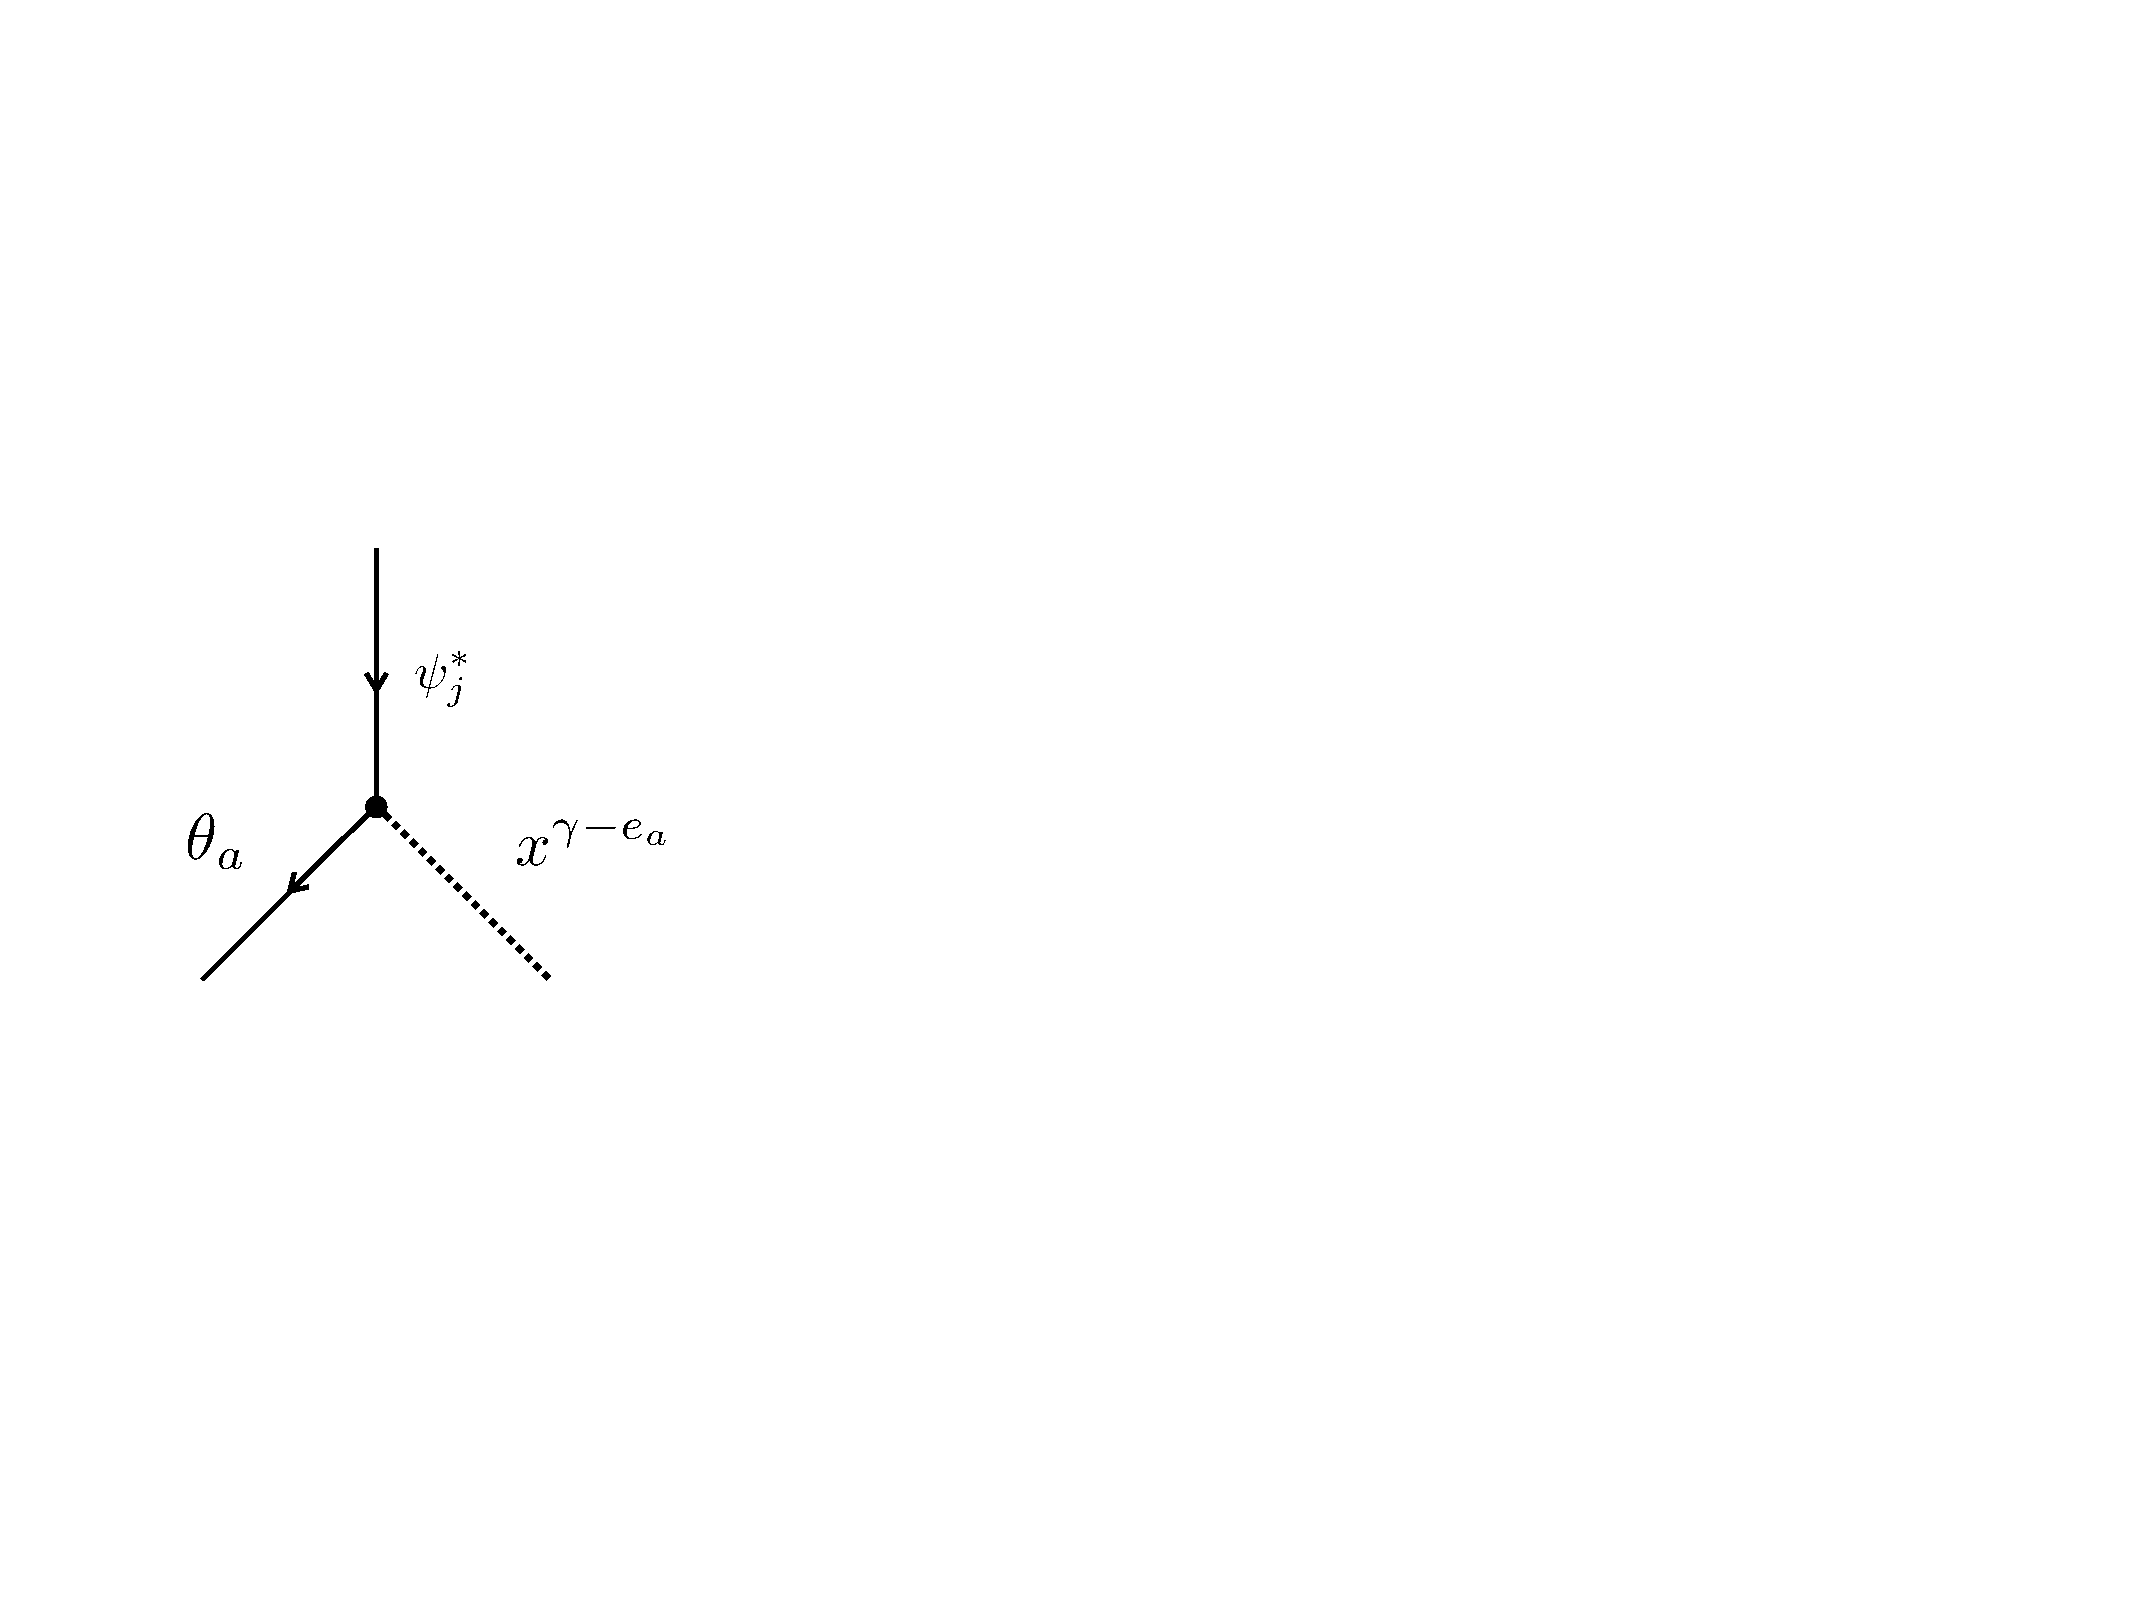
\includegraphics[scale=0.4]{dia2}
&
$\theta_a x^{\gamma - e_a} \big[\psi_j, -\big] \in \End_k( \mathscr{H} )$\\
\vspace{0.5cm}
$1 \le a,j \le n\,, \gamma \in \mathbb{N}^n$
&
\tagarray{\label{interaction_1}}
\end{tabular}
\end{center}

\begin{center}
\begin{tabular}{ >{\centering}m{1cm} >{\centering}m{4cm} >{\centering}m{8cm} >{\centering}m{1cm}}
\textbf{B}
&
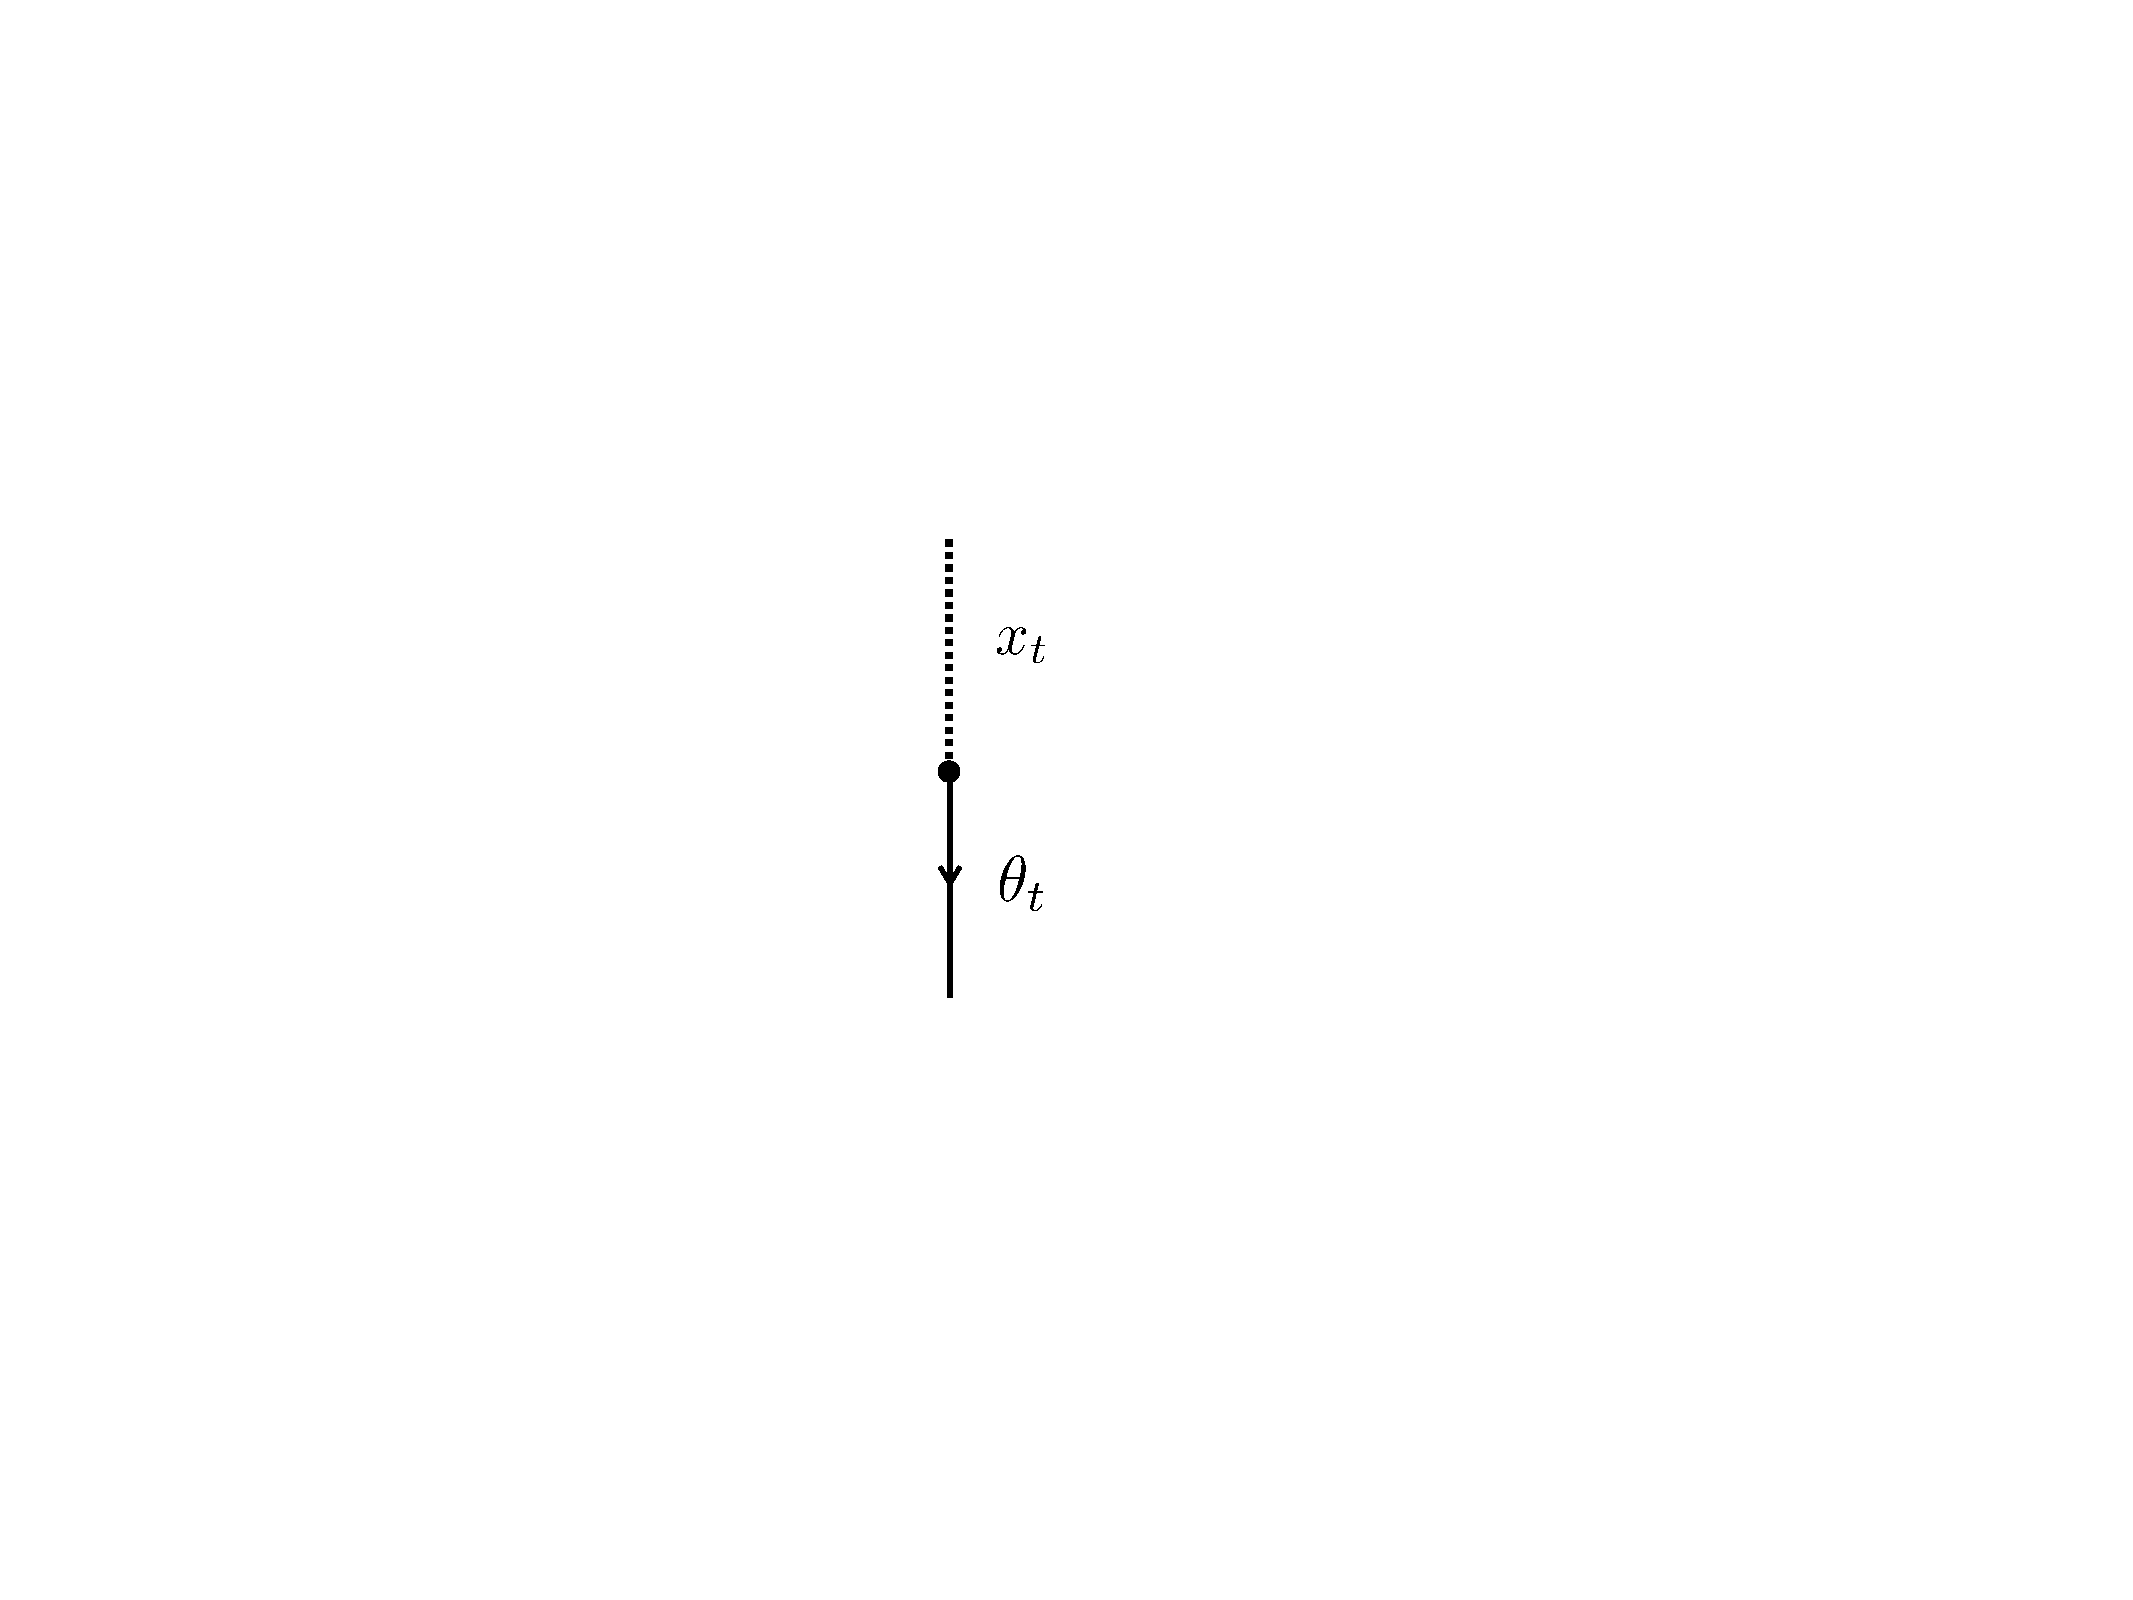
\includegraphics[scale=0.4]{dia3}
&
$\theta_t \partial_t \in \End_k( \mathscr{H} )$\\
\vspace{0.5cm}
$1 \le t \le n$
&
\tagarray{\label{interaction_2}}
\end{tabular}
\end{center}

\begin{center}
\begin{tabular}{ >{\centering}m{1cm} >{\centering}m{4cm} >{\centering}m{8cm} >{\centering}m{1cm}}
\textbf{C}
&
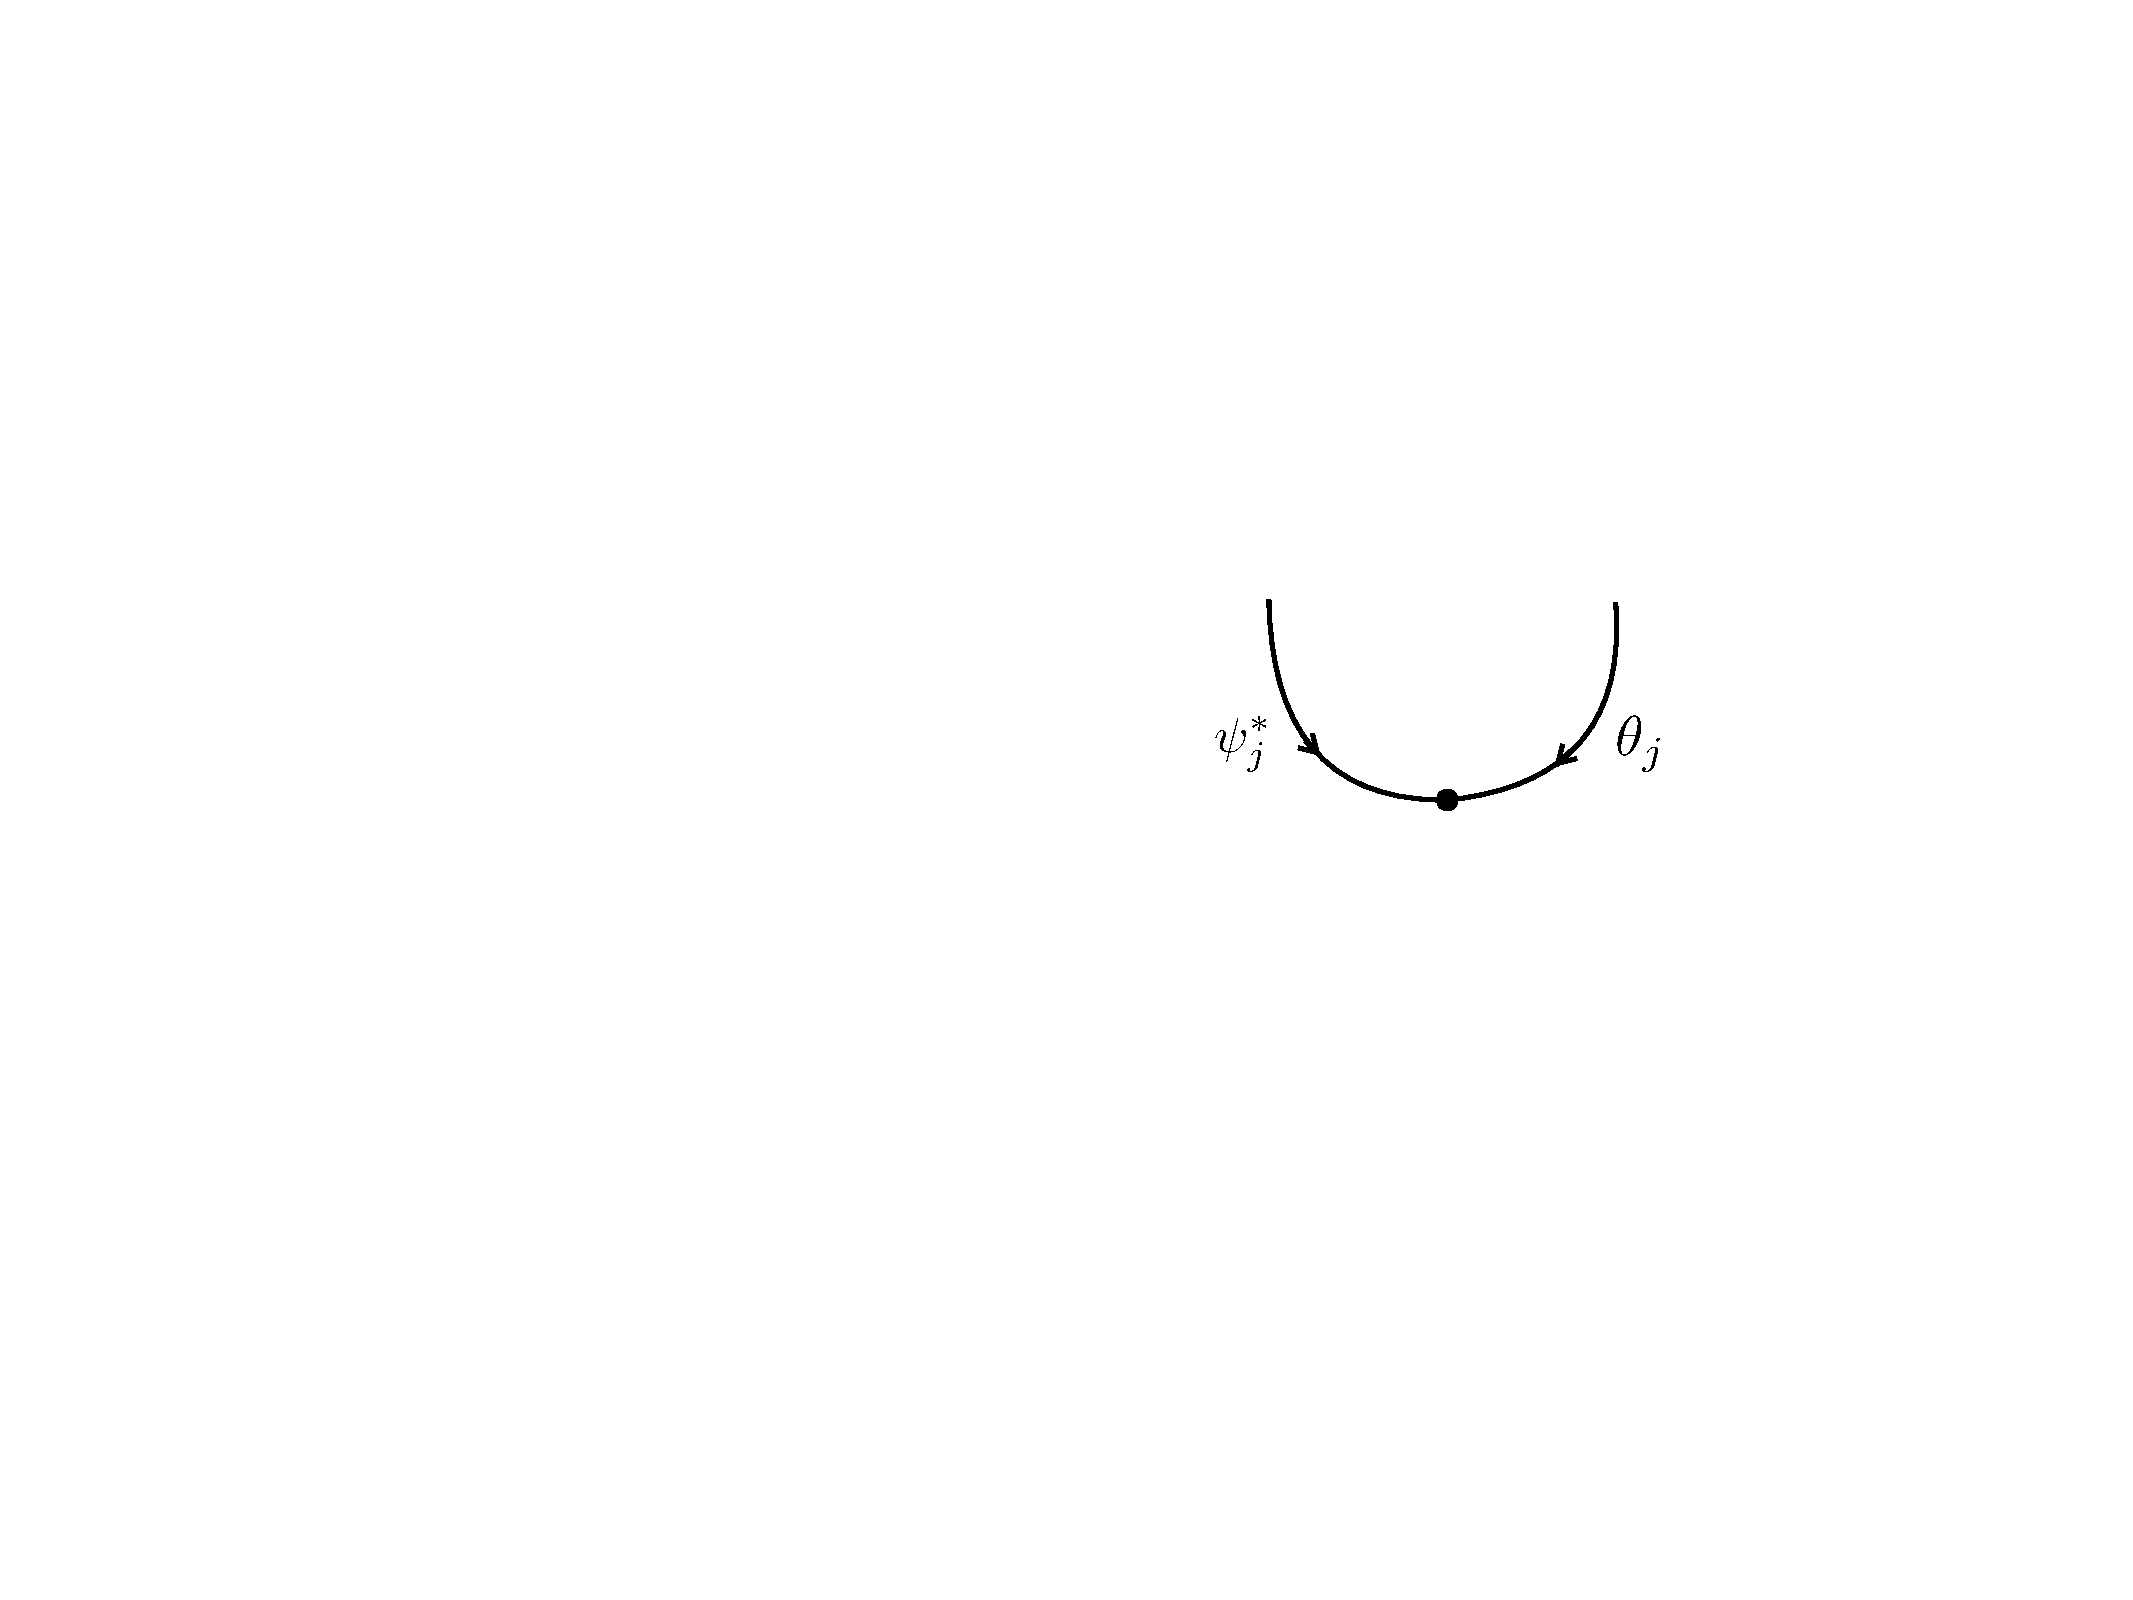
\includegraphics[scale=0.4]{dia4}
&
$m_2 \big( \big[\psi_j,-\big] \otimes \theta_j^* \big) \in \Hom_k( \mathscr{H}^{\otimes 2}, \mathscr{H} )$\\
\vspace{0.5cm}
$1 \le j \le n$
&
\tagarray{\label{interaction_3}}
\end{tabular}
\end{center}
Here $m_2$ is the multiplication in $\mathscr{H}$ and, given $\gamma \in \mathbb{N}^n$, we write $x^\gamma = x_1^{\gamma_1} \cdots x_n^{\gamma_n}$, with $e_i \in \mathbb{N}^n$ the unit vector with $x^{e_i} = x_i$. By convention if $\gamma_a = 0$ then $x^{\gamma - e_a} = 0$, which ensures that we always have $\gamma_a x^{\gamma - e_a} = \partial_a(x^\gamma)$. Finally note that bosons are depicted with dotted lines, and fermions with solid lines.

These interactions ``take place'' at vertices of the tree $A(T)$ for some $T \in \cat{T}_q$, and come with the following constraints, which will be formalised below in terms of combinatorial data called \emph{configurations}. We write $f(\gamma)$ for the coefficient of $x^\gamma$ in a polynomial $f \in R$ and recall the chosen decomposition $W = \sum_j x_j W^j$. 

\begin{itemize}
\item A-type interactions only occur at input vertices and internal edges of $T$. 
\item B-type interactions only occur at internal edges of $T$.
\item C-type interactions only occur at internal vertices of $T$, and moreover the incoming lines must come from different branches of the tree.
\item There may be arbitrarily many A-type or C-type interactions per vertex of $A(T)$, but there is \emph{precisely one} B-type interaction at each internal edge of $T$.
\item The A-type interaction with indices $a,j, \gamma$ appears with the coefficient
\be\label{eq:coeff_a}
-\frac{\gamma_a}{|\gamma|} W^j( \gamma)\,.
\ee
where $|\gamma| = \sum_{i=1}^n \gamma_i$. Each B- and C-type interaction appears with coefficient $(-1)$.
\end{itemize}

As we will see, the coefficient \eqref{eq:coeff_a} is the only way that $W$ enters the rules, and thus the definition of the $A_\infty$-products on $\mathscr{B}$. The precise definition of the Feynman rules will be given in Definition \ref{defn:config} below, but first we give an example of a tree with interactions inserted, to illustrate the various ingredients.

\begin{example}\label{ex:picture_example} Consider the tree $T \in \cat{T}_3$ whose augmented tree $A(T)$ is depicted below, together with labels for its vertices, where we label by $e$ the vertex corresponding to the internal edge of $T$:
\begin{center}
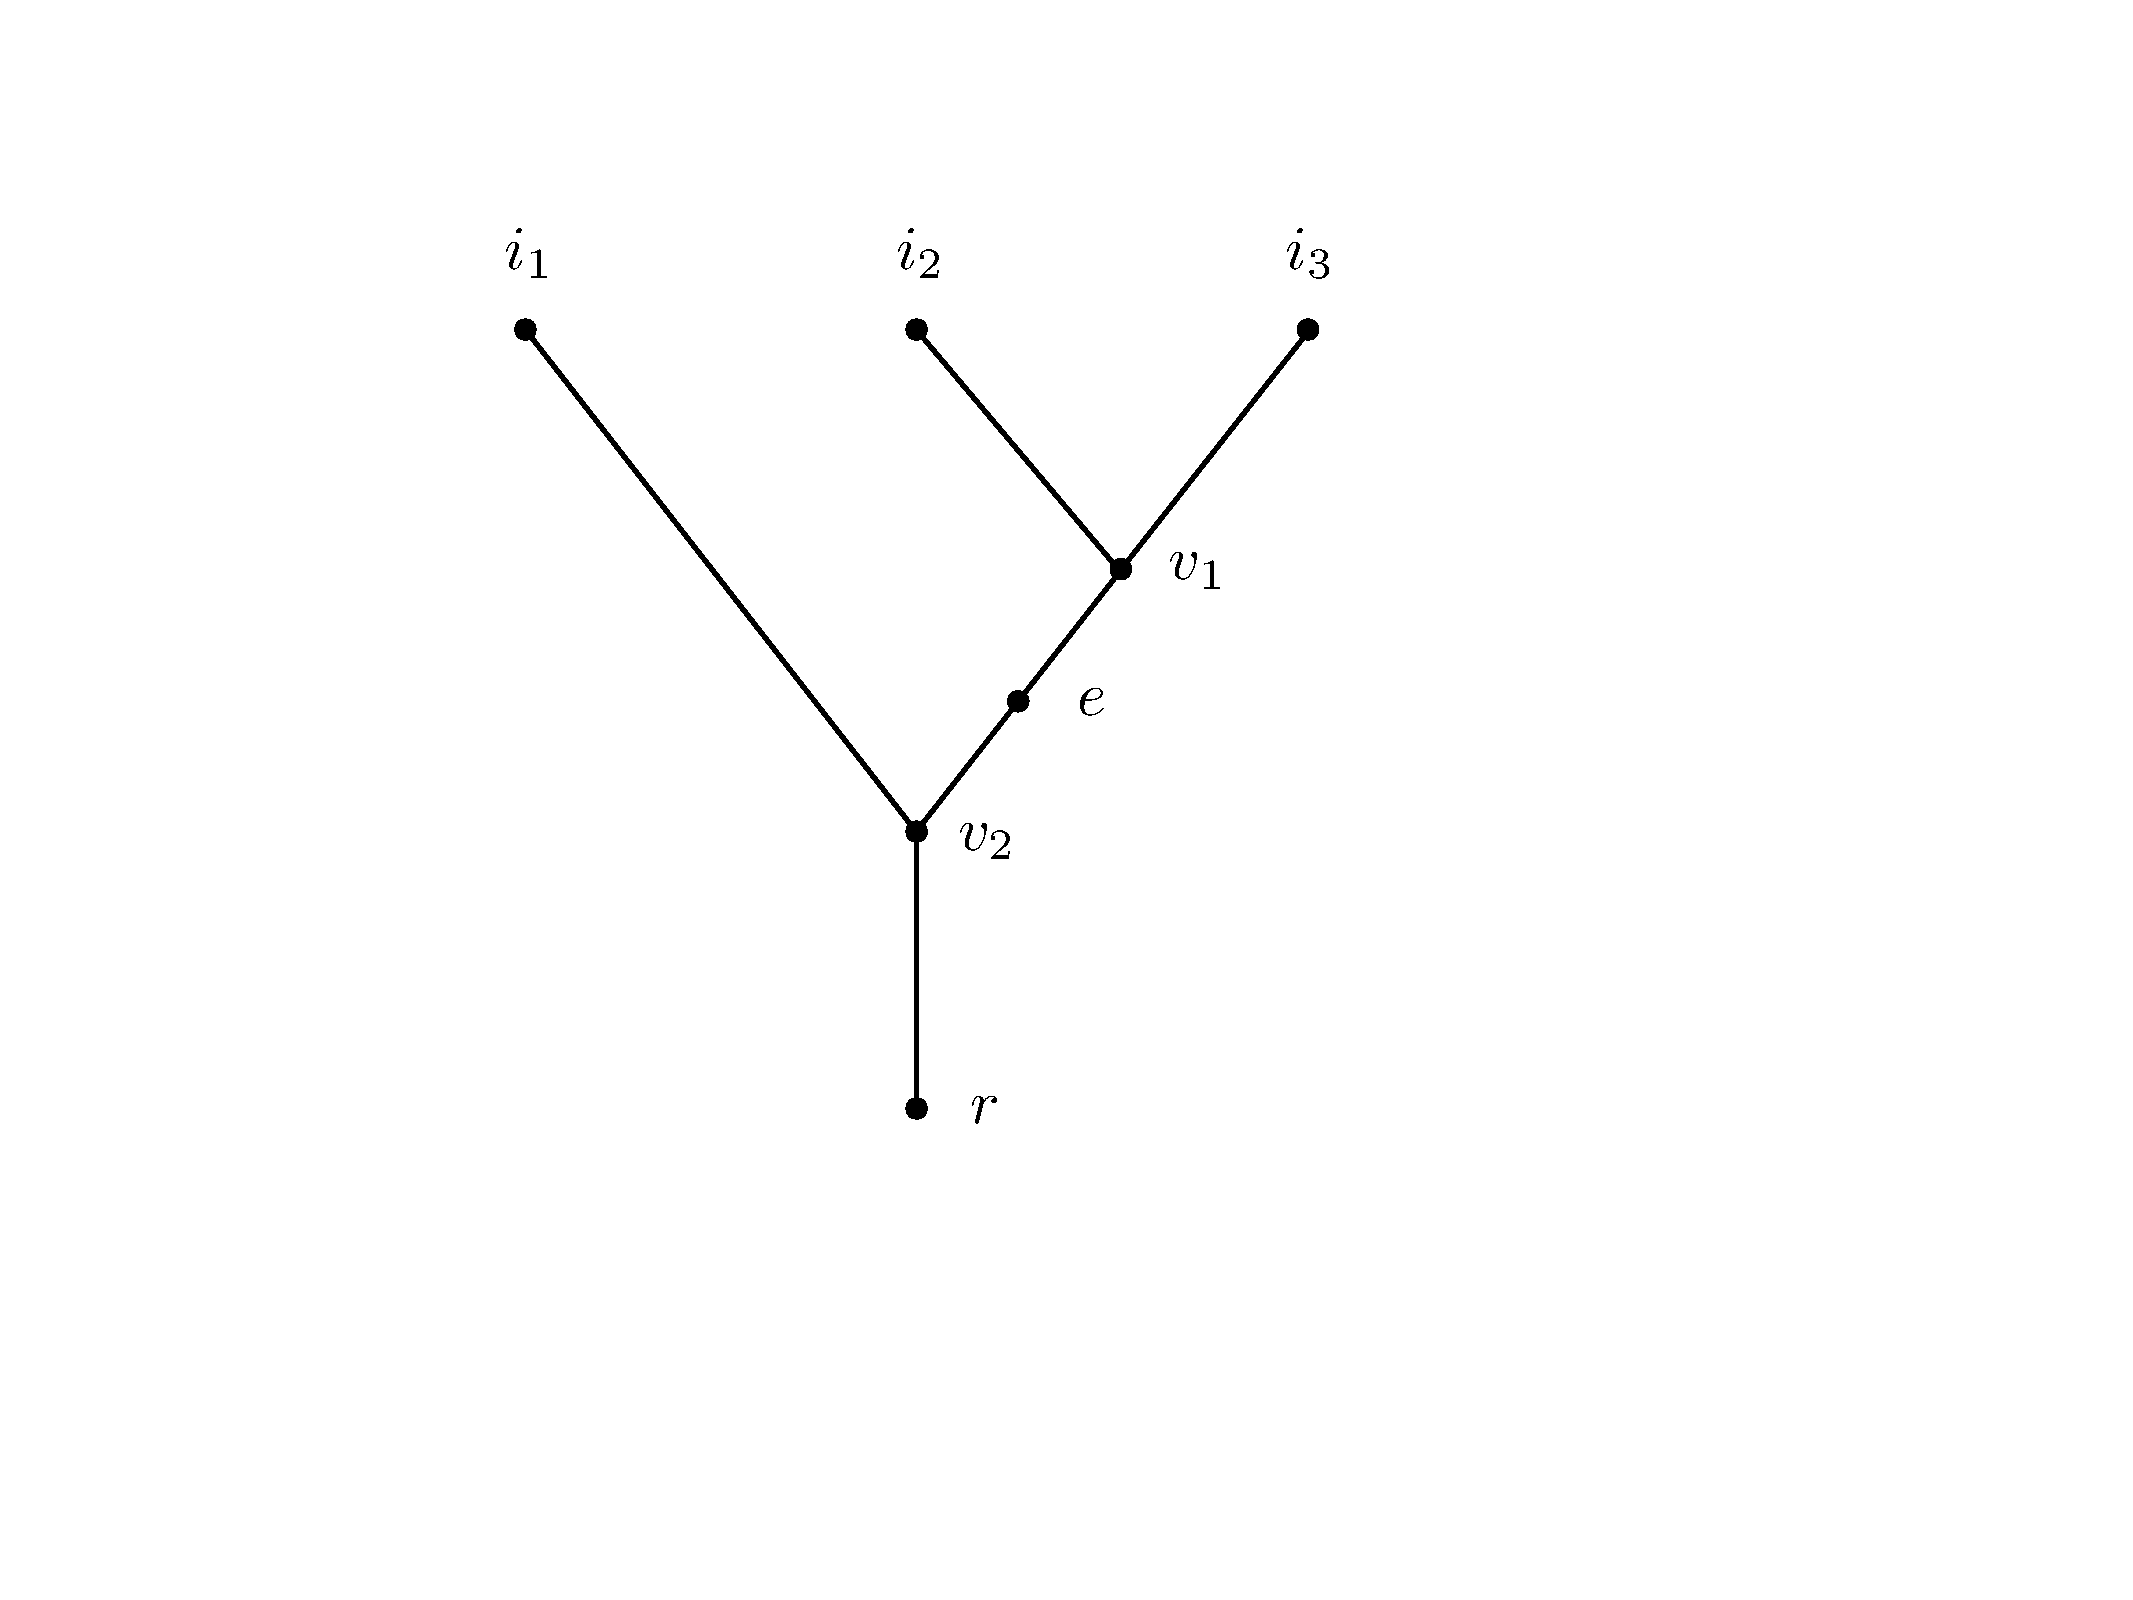
\includegraphics[scale=0.25]{dia7}
\end{center}
Set $W = x^3 \in \mathbb{C}[x]$ so that $W^1 = x^2$ and the only A-type interaction has $a = 1, j = 1, \gamma = 2$ and coefficient $-1$, as in the diagram (we write $\theta = \theta_1, \psi = \psi_1$)
\begin{center}
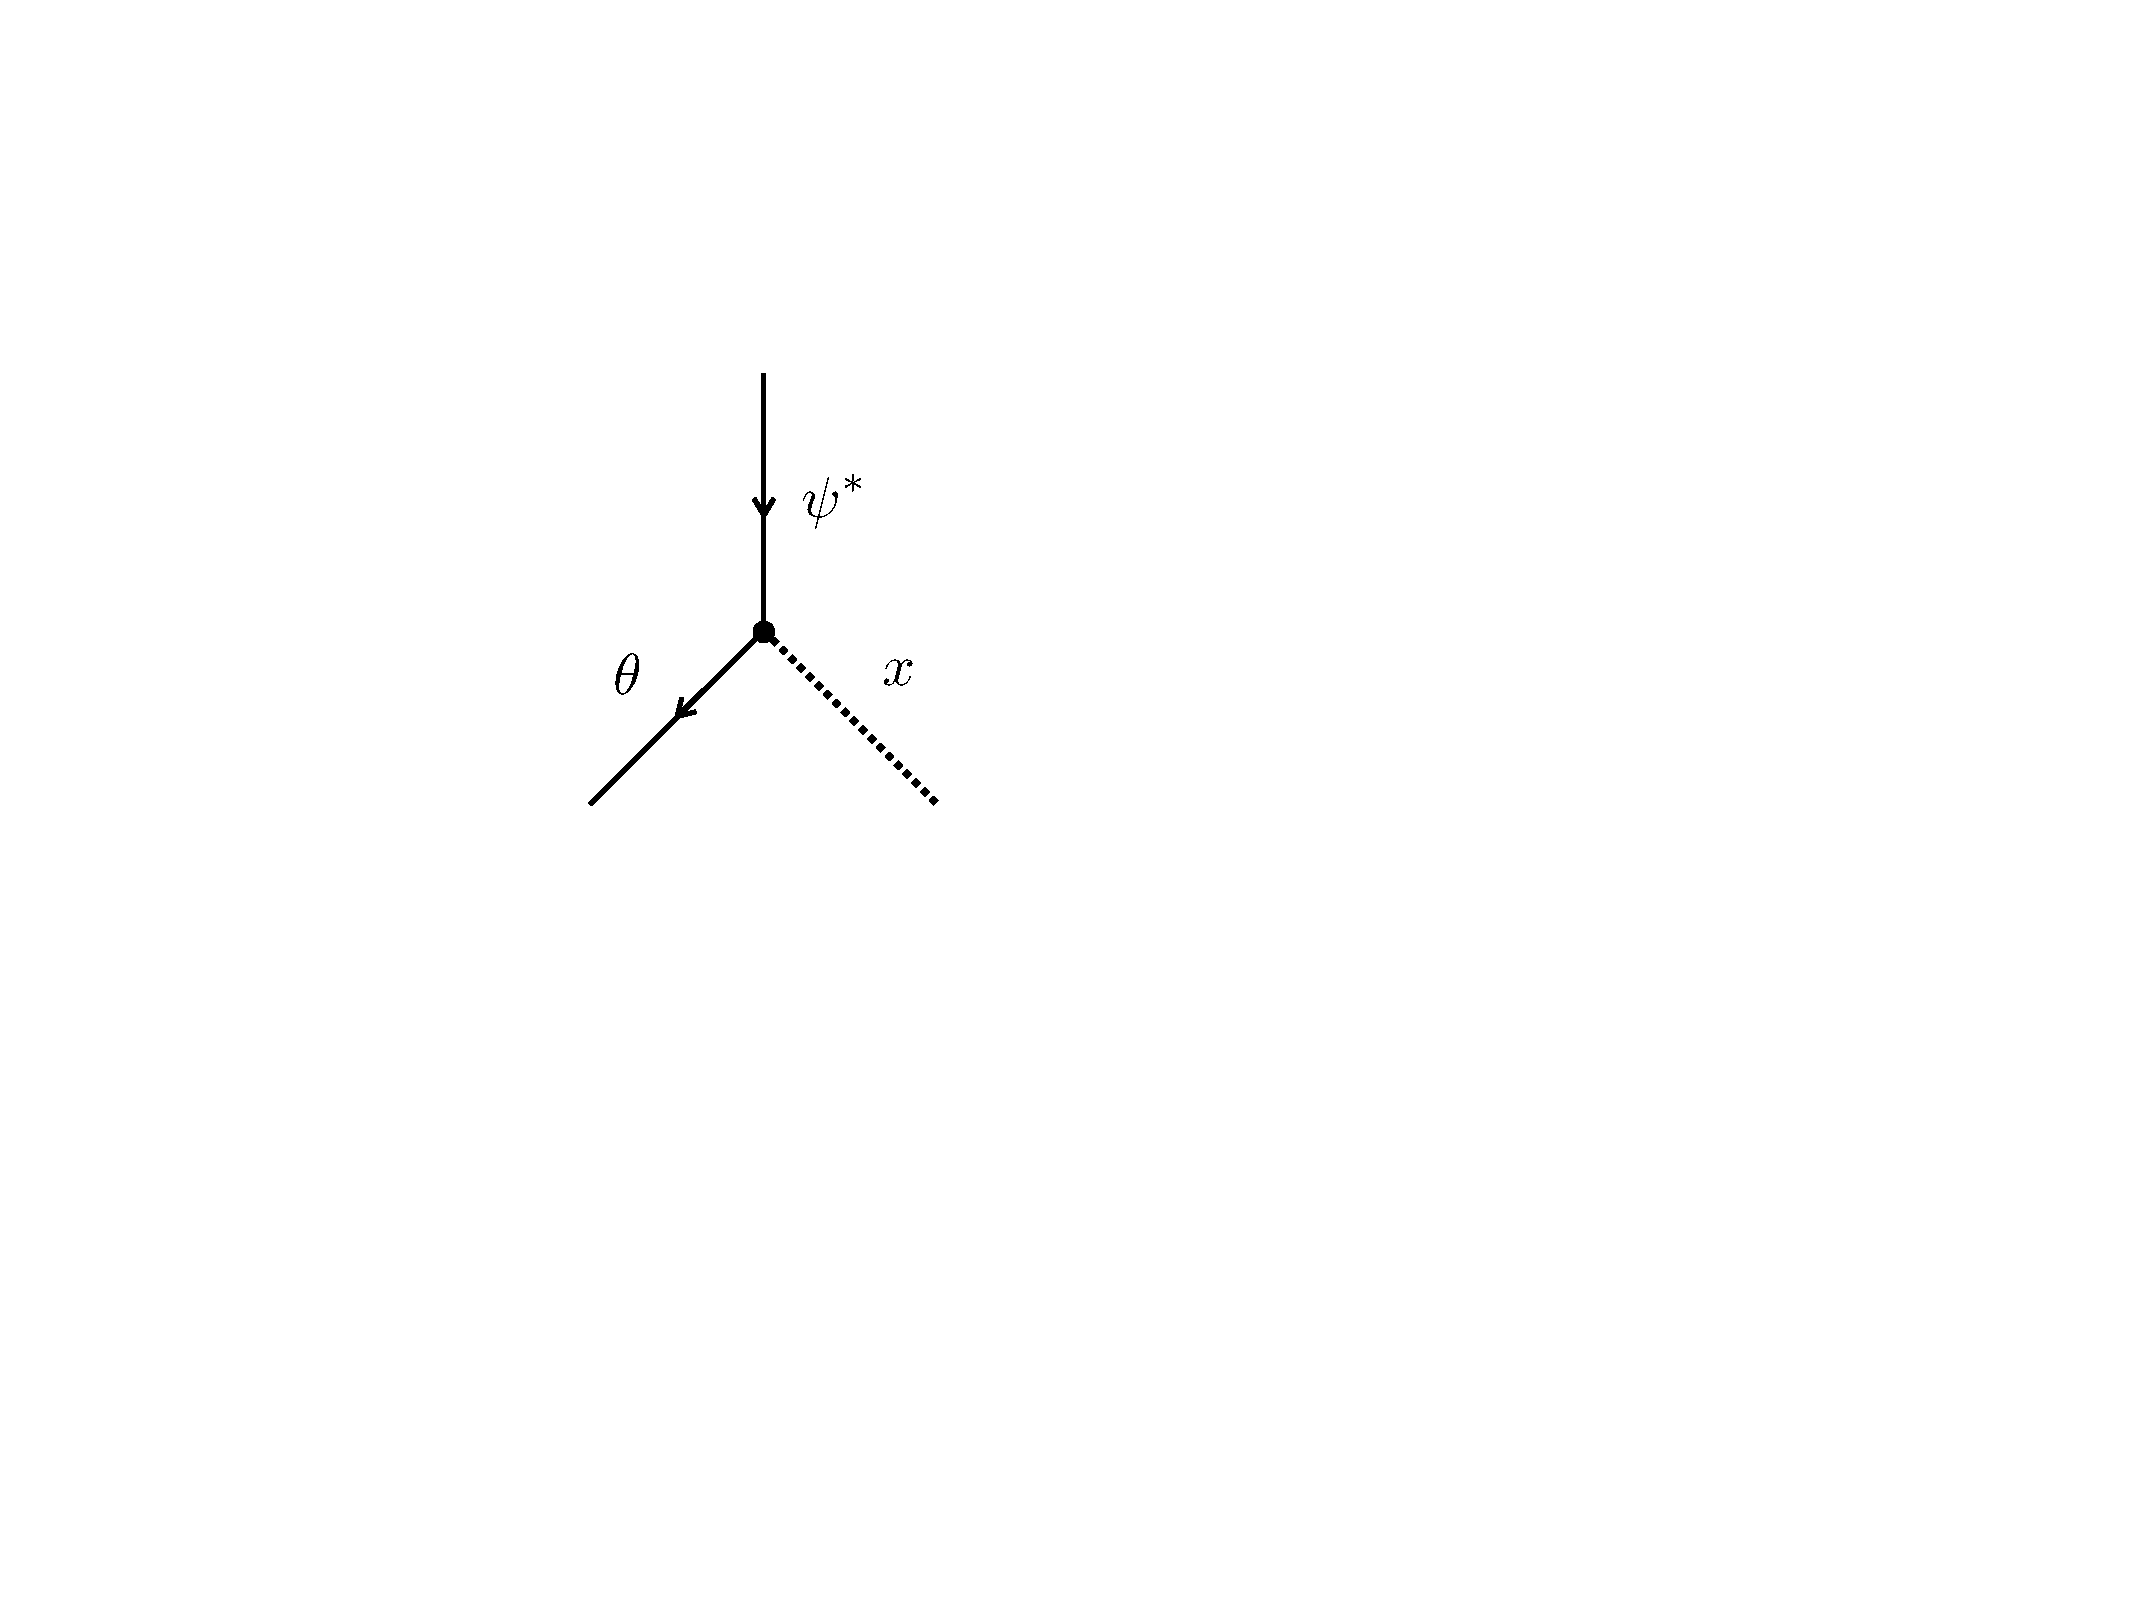
\includegraphics[scale=0.3]{dia5}
\end{center}
Consider the input state $\Psi = \psi^* \otimes \psi^* \otimes \psi^*$ in $\mathscr{B}^{\otimes 3}$. One possible pattern of interactions (called a configuration, below) has a single A-type interaction at the input vertex $i_3$, a B-type interaction at $e$, and two C-type interactions at $v_1,v_2$, as shown in the following ``topological'' Feynman diagram
\begin{center}
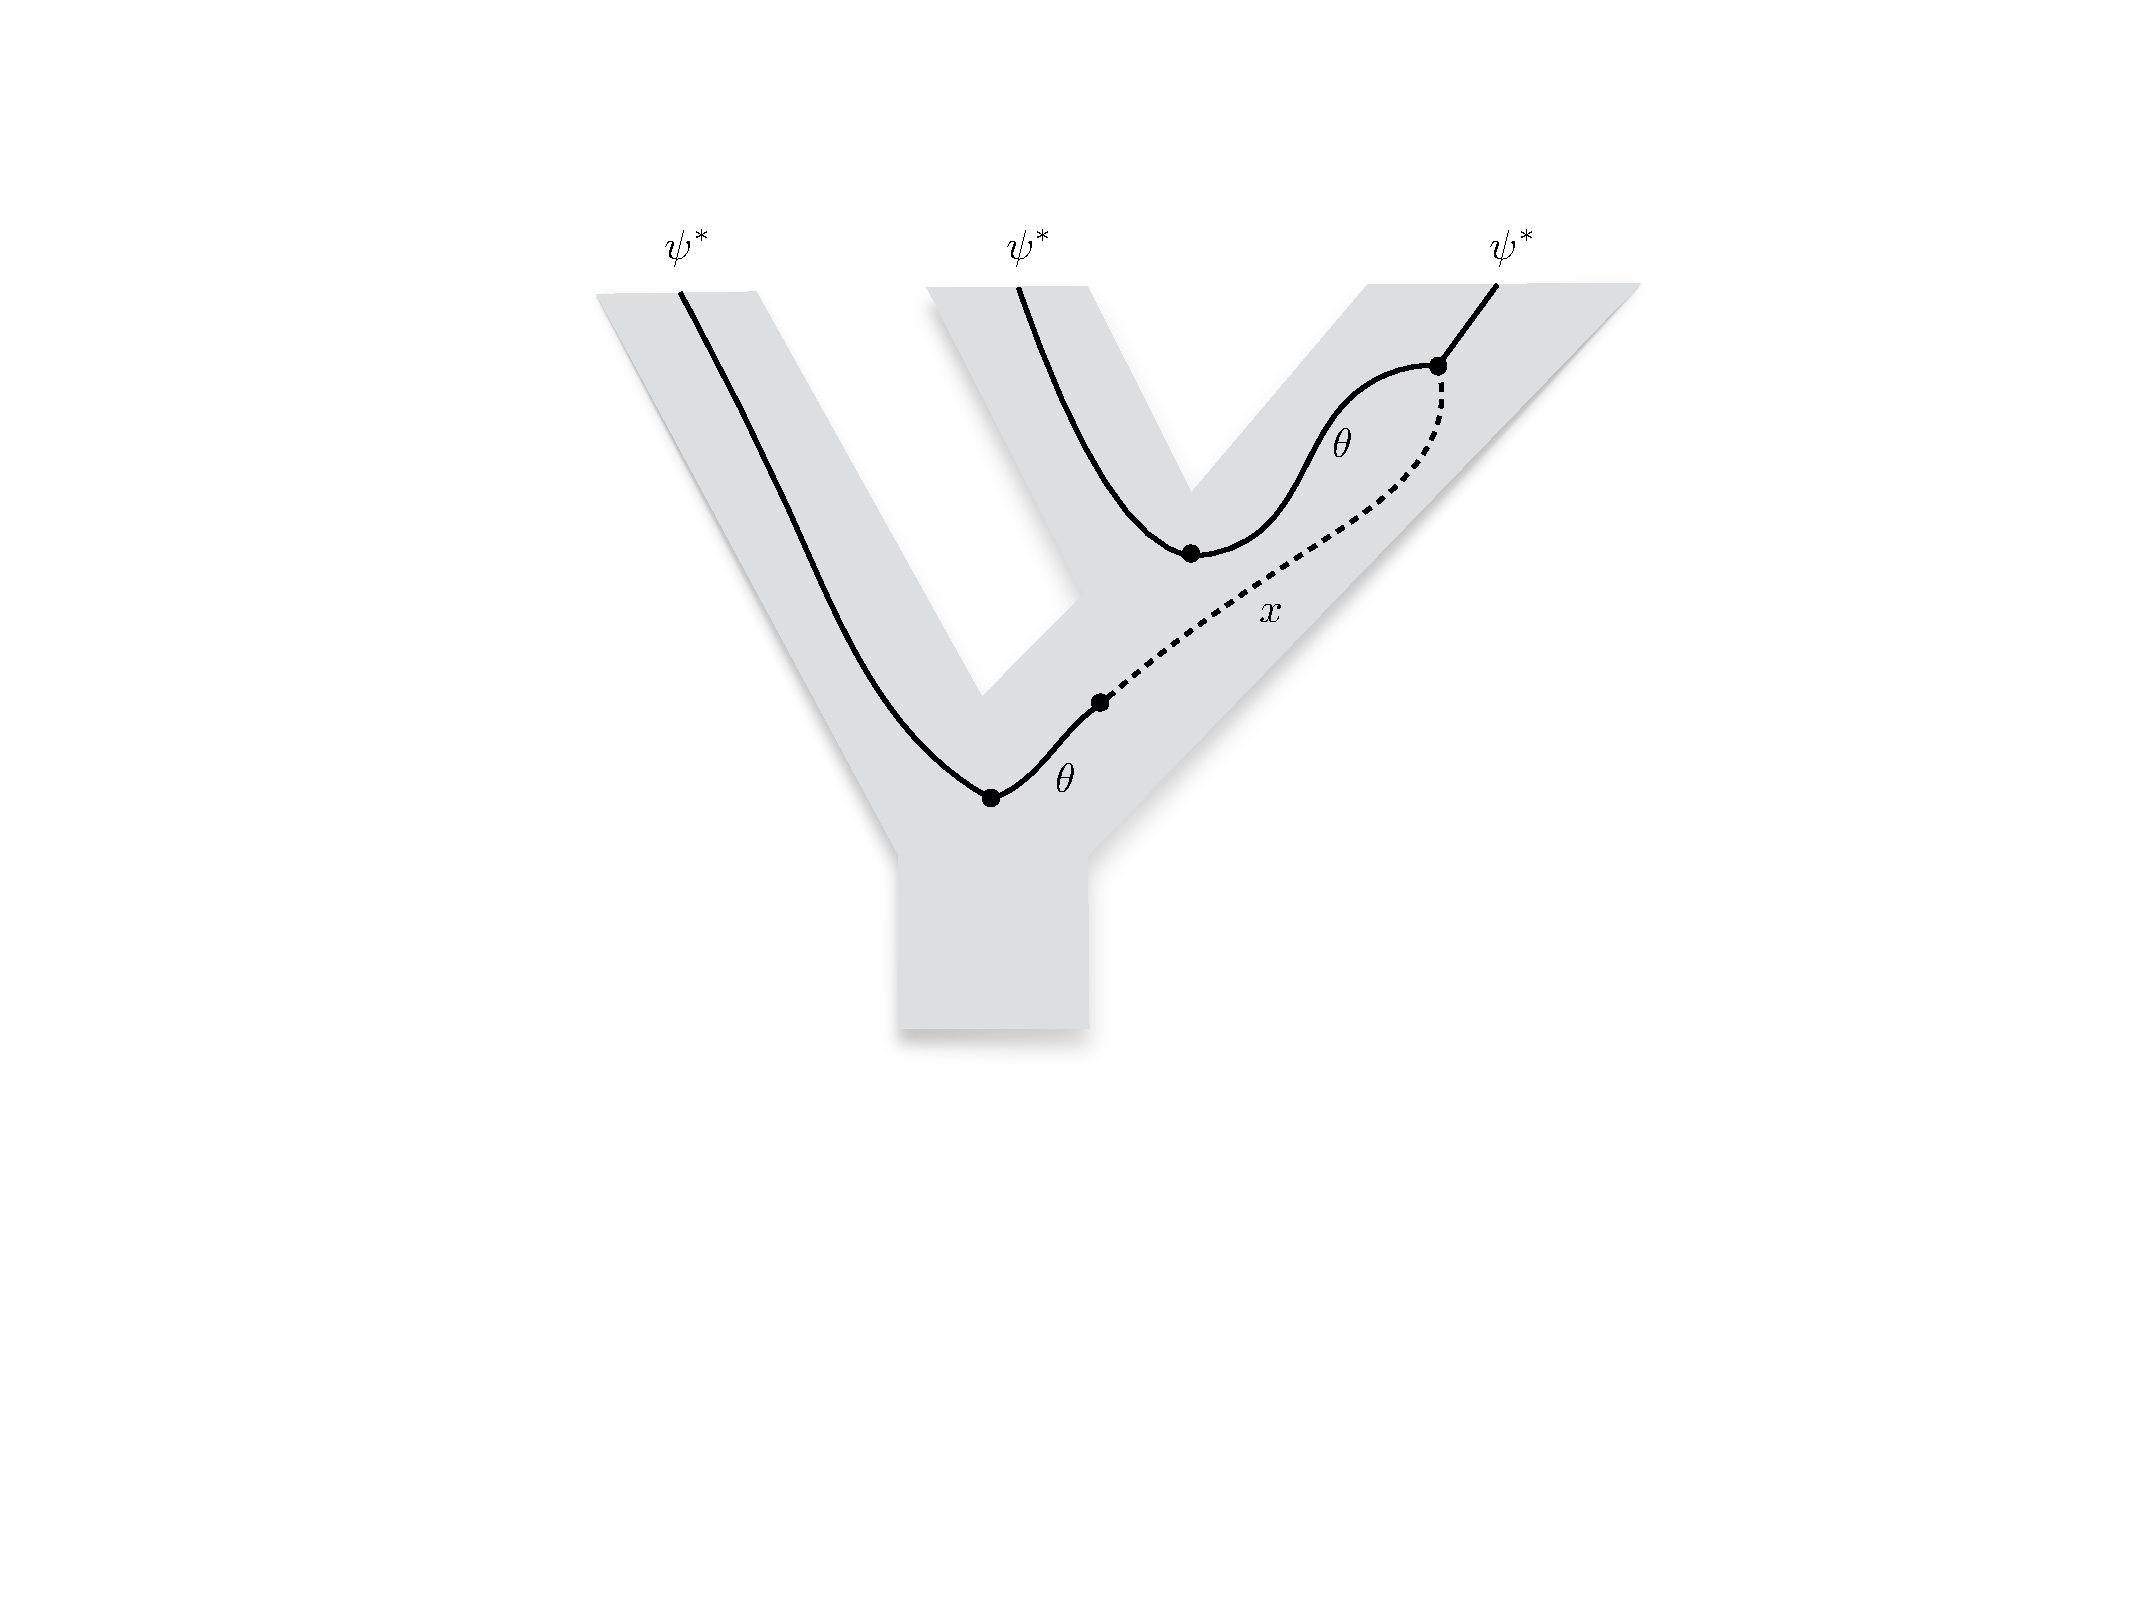
\includegraphics[scale=0.3]{dia6}
\end{center}
The \emph{value} of this diagram is the value of the linear map
\be\label{eq:operator_tree_example}
(-1)^3 p \circ m_2 \big([\psi, -] \otimes \theta^*\big) \circ \big( \iota \otimes \theta \partial_x \circ m_2 ([\psi, -] \otimes \theta^*)\big( \iota \otimes \theta x [\psi, -] \iota \big)\big)
\ee
on the input state $\Psi$. Usually when evaluating such an expression we would pay attention to Koszul signs from commuting the input $\psi^*$'s into position (see Definition \ref{??}). Ignoring all signs, the value is
\begin{align*}
\pm \; & p \circ m_2 \big([\psi, -] \otimes \theta^*\big) \circ \big( \iota \otimes \theta \partial_x \circ m_2 ([\psi, -] \otimes \theta^*)\big( \iota \otimes \theta x [\psi, -] \iota \big)\big)\Big( \Psi \Big)\\
&= \pm \; p \circ m_2 \big([\psi, \psi^*] \otimes \theta^* \theta \partial_x \circ m_2 ([\psi, \psi^*] \otimes \theta^* \theta x [\psi, \psi^*] \big)\big)\\
&= \pm \; p \circ m_2 \big(1 \otimes \theta^* \theta \partial_x \circ m_2 (1 \otimes \theta^* \theta x \big)\big)\\
&= \pm \; p \circ m_2 \big(1 \otimes \partial_x(x) \big)\\
&= \pm \; p(1) = \pm \; 1 \in \mathscr{H}\,.
\end{align*}
\end{example}

Now we give some more precise definitions. Let $T \in \cat{T}_q$ be a valid plane tree with $q$ inputs and $e_i(T)$ internal edges, and let $A(T)$ be the augmented plane tree. The definitions are all relative to the ambient integer $n$, but for the sake of readability we will not reflect this in the notation.

\begin{definition}\label{defn:config} A \emph{configuration} $C$ of a valid plane tree $T$ consists of the following data, for each non-root vertex $v$ of $A(T)$:
\begin{itemize}
\item An integer $m(v) \ge 0$.
\item A subset $J(v) \subseteq \{ 1,\ldots, n \}$ with $|J(v)| = m(v)$. 
\item If $v$ is an input, or comes from an internal edge of $T$, a pair
\[
( a_j(v), \gamma_j(v) ) \in \{ 1, \ldots, n \} \times \mathbb{N}^n
\]
for each $j \in J(v)$, with $\gamma_j(v)_{a_j(v)} \ge 1$.
\item If $v$ comes from an internal edge of $T$, an integer $t(v) \in \{1,\ldots,n\}$.
\end{itemize}
Let $\operatorname{Con}(T)$ denote the set of all configurations.
\end{definition} 

\begin{remark} The integer $m(v)$ counts how many interactions of type A or C take place at $v$ (there is no point counting B interactions as precisely one occurs at each internal edge). The set $J(v)$ consists of all $j$-indices appearing in interactions at $v$. The interactions of A-type (at inputs and internal edges) are defined by indices $a_j(v), \gamma_j(v)$ while at each internal edge $e$ of $T$, $t(e)$ is the index of the B-type interaction.
\end{remark}

\begin{definition} Given a tree $T \in \cat{T}_q$ and configuration $C \in \operatorname{Con}(T)$ we define a decoration $D_{T,C}$ of $A(T)$ by the assignment of the modules
\begin{itemize}
\item $\mathscr{B}$ to the input at each non-root leaf, and
\item $\mathscr{H}$ to each edge and the output at the root.
\end{itemize}
To each vertex $v$ of $A(T)$ we associate an operator $\phi_v$ as follows, writing $m, J, \{ (a_j, \gamma_j) \}_{j \in J}, t$ for the data associated to $v$ by the configuration $C$:
\begin{itemize}
\item if $v$ is an input, then $\phi_v$ is the linear map $\mathscr{B} \lto \mathscr{H}$ given by
\be\label{eq:int_input}
\phi_v = (-1)^m \prod_{j \in J}\Big\{ \frac{1}{|\gamma_j|}(\gamma_j)_{a_j} W^j( \gamma_j)  \theta_{a_j} x^{\gamma_j - e_{a_j}} \big[ \psi_j, - \big] \Big\} \circ \iota\,.
\ee
Note that the operator under the product is even, so the order is irrelevant. If $J(v)$ is empty then the product is interpreted to be the identity operator.
\item if $v$ comes from an internal edge of $T$, then
\be\label{eq:int_intedge}
\phi_v = (-1)^m \prod_{j \in J} \Big\{ \frac{1}{|\gamma_j|}(\gamma_j)_{a_j} W^j( \gamma_j)  \theta_{a_j} x^{\gamma_j - e_{a_j}} \big[ \psi_j, - \big] \Big\} \circ \theta_t \partial_t\,.
\ee
\item if $v$ comes from an internal vertex of $T$, then
\be\label{eq:int_intvert}
\phi_v = (-1)^m m_2 \circ \prod_{j \in J} \Big\{ \big[ \psi_j, - \big] \otimes \theta_j^* \Big\}
\ee
which is a map $\mathscr{H}^{\otimes 2} \lto \mathscr{H}$. Here $m_2$ denotes the product on $\mathscr{H}$.
\item if $v = r$ is the root, $\phi_v = p: \mathscr{H} \lto \mathscr{H}$ is the projection of Definition \ref{defn:handop}.
\end{itemize}
\end{definition}

The denotation $\langle D_{T,C} \rangle$ of this decoration is \emph{a priori} a linear map $\mathscr{B}^{\otimes q} \lto \mathscr{H}$, but since the only operators in the decoration acting on the third tensor factor of $\mathscr{H}$ in \eqref{eq:defnH} are the commutators $[\psi_i,-]$ under which $\mathscr{B}$ is closed, $\langle D_{T,C} \rangle$ actually has its image contained in the submodule $\mathscr{B} \subseteq \mathscr{H}$. 

\begin{definition}\label{defn:otc} Given $T \in \cat{T}_q$ and $C \in \operatorname{Con}(T)$ we define the $k$-linear operator
\[
\cat{O}(T, C): \mathscr{B}^{\otimes q} \lto \mathscr{B}
\]
to be the denotation $\cat{O}(T,C) = \langle D_{T,C} \rangle$, defined without Koszul signs.
\end{definition}

\begin{example}\label{ex:picture_example_2} The configuration $C$ which is described in Example \ref{ex:picture_example} has $n = 1$ and
\begin{gather*}
m(i_3) = m(v_1) = m(v_2) = 1\,,\\
J(i_3) = J(v_1) = J(v_2) = \{ 1 \}\,,\\
t(e) = 1\,.
\end{gather*}
At $i_3$ we have the pair $a = 1$ and $x^\gamma = x^2$. The operator $\cat{O}(T,C)$ is precisely \eqref{eq:operator_tree_example}.
\end{example}

\begin{remark} Let us now briefly explain the connection between configurations, the linear map $\cat{O}(T,C)$ and Feynman diagrams, such as the one in Example \ref{ex:picture_example}. Ultimately we will not actually use these diagrams to perform calculations, so we refrain from formulating them too precisely; however, they are very useful as a tool for understanding.

We view $\Psi_1 \otimes \cdots \otimes \Psi_q \in \mathscr{B}^{\otimes q}$ as the result of applying creation operators (meaning wedge products $\psi_i^* \wedge -$) to the vacuum (meaning the identity of the exterior algebra) in the various copies of $\mathscr{B}$. The value of $\cat{O}(T,C)$ on $\Psi$ may be computed by commuting all creation operators acting on $\mathscr{H}$ (that is, the operators $x_i, \theta_i, \psi_i^*$) leftward in the expression, which means \emph{down} the tree. These operators commute with all other creation operators and with those annihilation operators that are either of a different type (e.g. $[x_i, \theta_j^*] = 0$) or of same type but with different indices (e.g. $[x_1, \partial_2] = 0$). However, there will be a nonzero commutator every time a creation operator meets an annihilation operator of the same type and index (respectively $\partial_i, \theta_i^*, [\psi_i, -]$). We view such a commutator, say
\[
\theta_i \theta_i^* + \theta_i^* \theta_i = [ \theta_i, \theta_i^* ] = 1\,,
\]
which arises as the result of commuting the $\theta_i$ leftward to meet the $\theta_i^*$, as generating two diagrams, corresponding to the two choices of summands in $\theta_i^* \theta_i = 1 - \theta_i \theta_i^*$. Choosing the first summand means there is an interaction (drawn as a line marked $\theta_i$ from the original position of the $\theta_i$ to the position of the $\theta_i^*$ in the tree) while choosing the second summand means there is no interaction (the $\theta_i$ sails on, to meet its partner further down the tree). If a particular series of choices leads to an $x_i$ or $\theta_i$ meeting the bottom of the tree then this diagram does not contribute to $\cat{O}(T,C)(\Psi)$ since $p$ projects out such elements of $\mathscr{H}$. 

We can depict a series of choices by linking the creation and annihilation operators,
\begin{center}
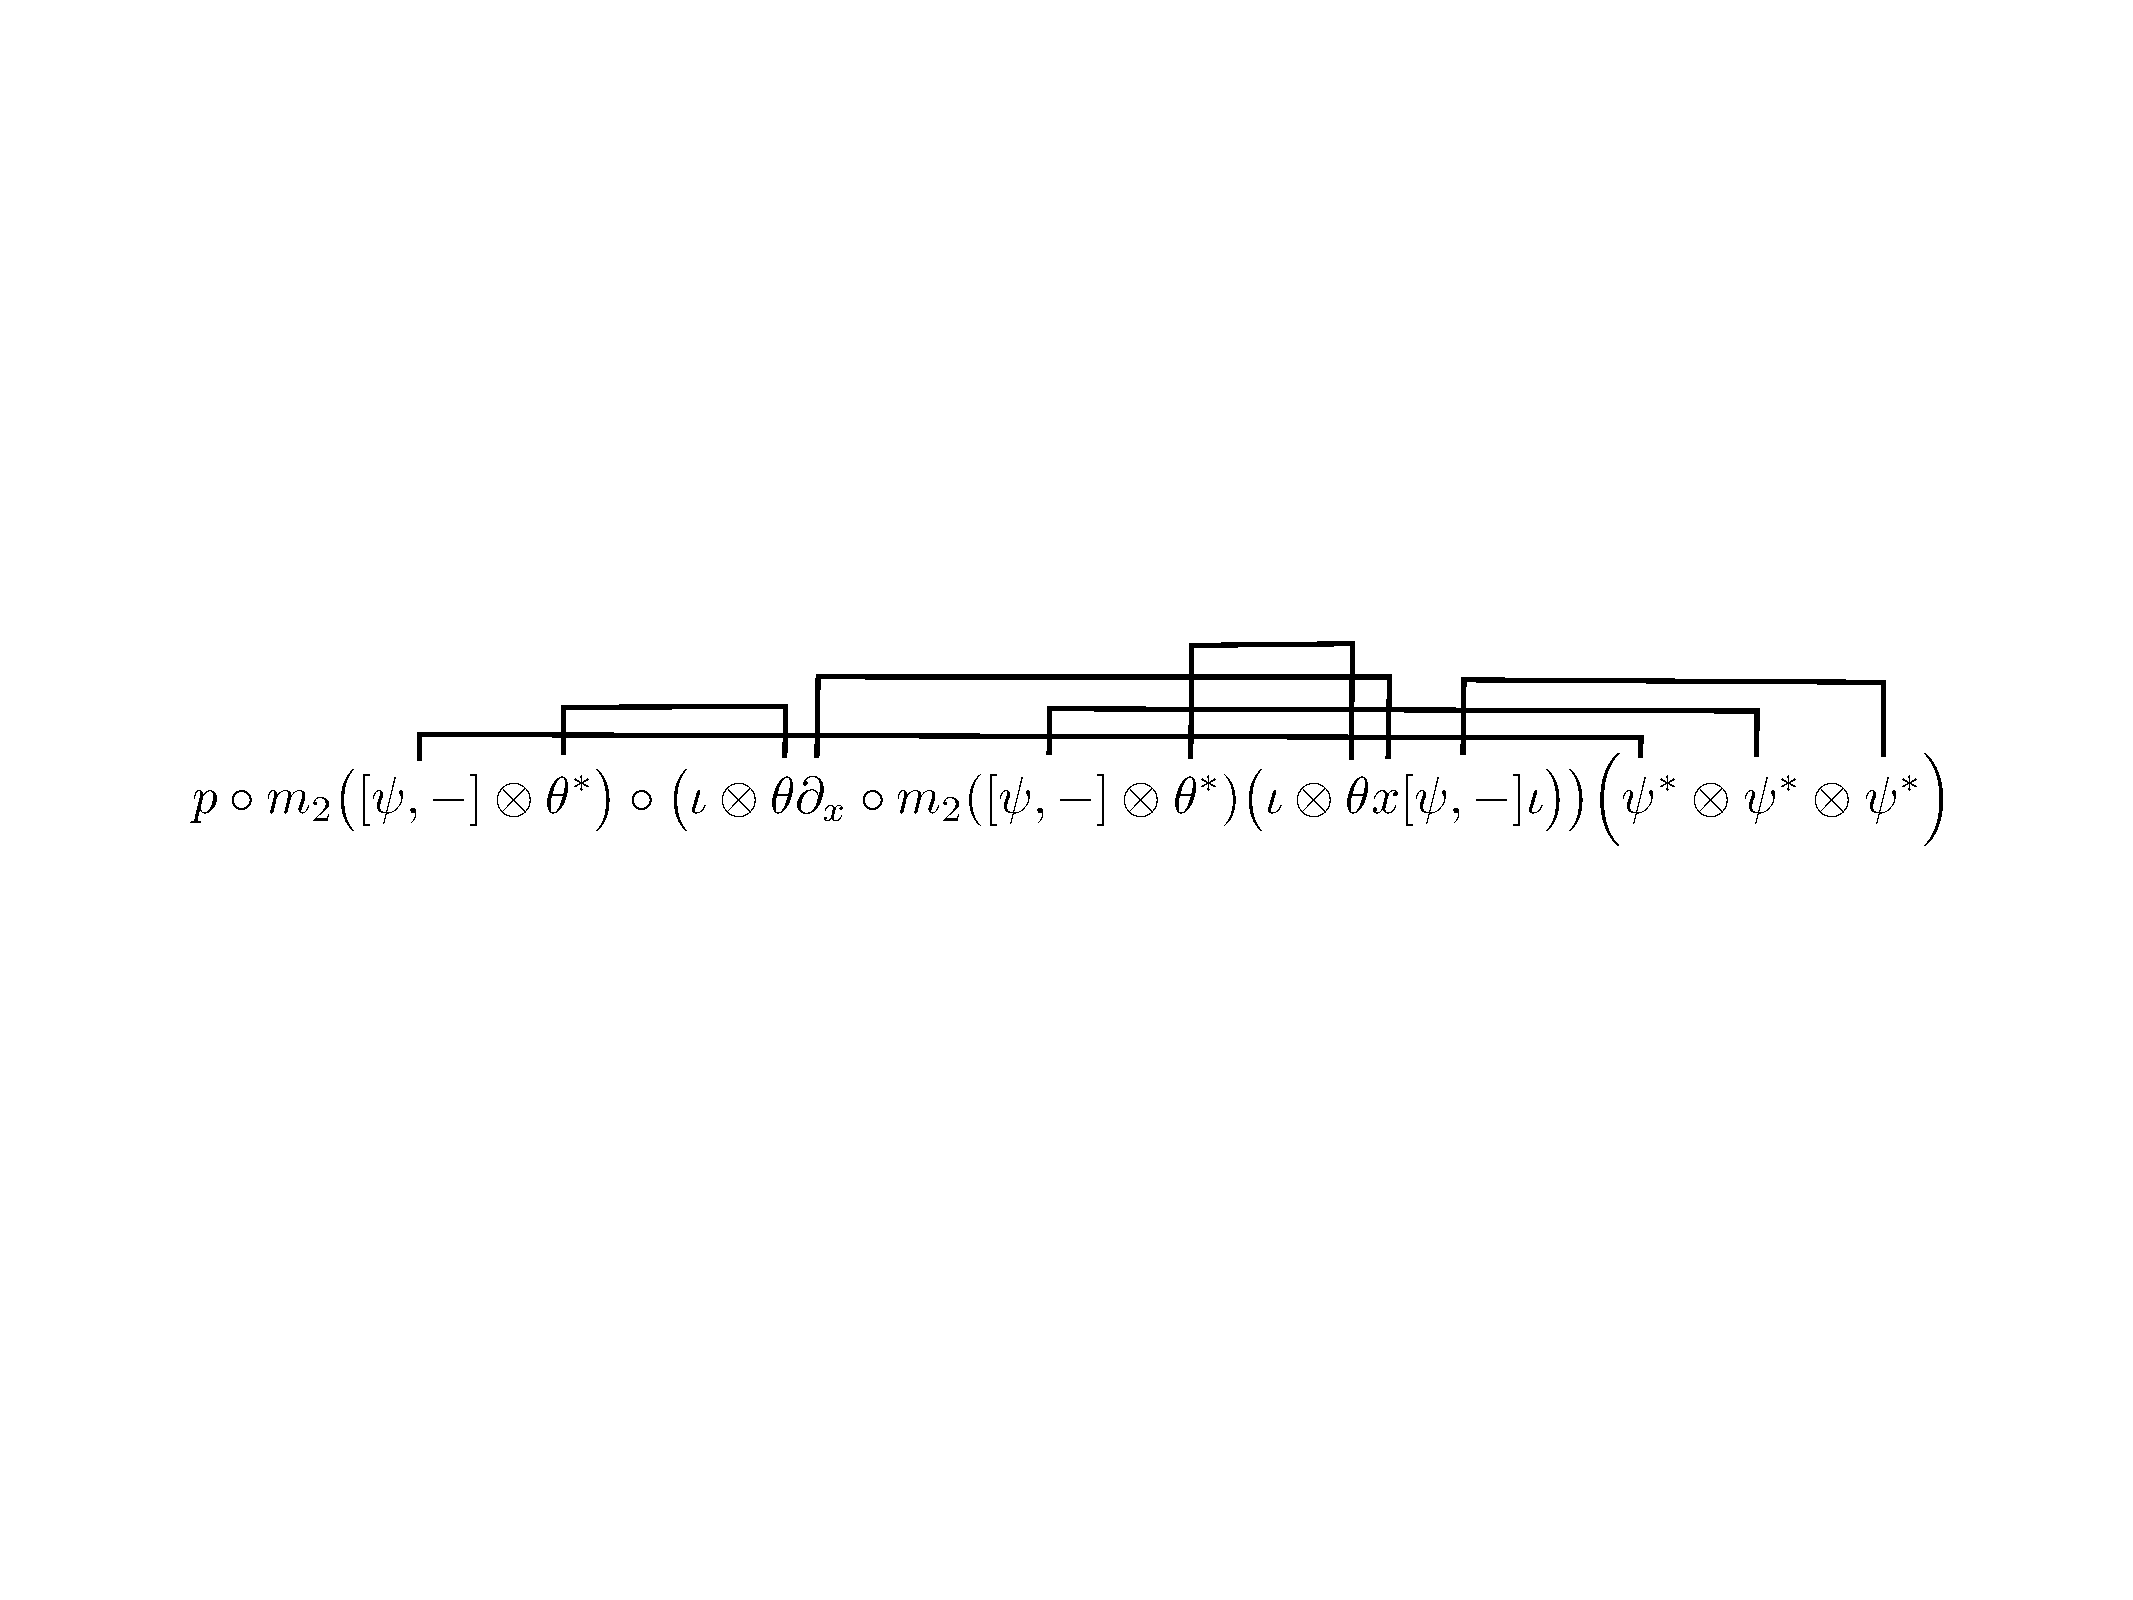
\includegraphics[scale=0.45]{dia8}
\end{center}
or by drawing these linkages, marked with the type and index of the ``particle'' on the tree $T$, joining the two positions determined by the configuration as in Example \ref{ex:picture_example}.

Note that in this example one of the other series of ``choices'' would involve commuting the rightmost $\theta$ past the first $\theta^*$ to meet with the leftmost $\theta^*$. In the corresponding Feynman diagram the $\theta$ fermion would travel from the A-type interaction vertex all the way to the bottom of the tree. However, this diagram gives a zero contribution to $\cat{O}(T,C)(\Psi)$, for at least two reasons: firstly, in the calculation we see parallel identical fermion lines which vanish (since $\theta^2 = 0$), and secondly the leftmost $\theta$ may in this case be commuted left to give zero on $p$, after the ``guard'' $\theta^*$ is cancelled by the other $\theta$.
\end{remark}

\begin{remark}\label{remark:virtual_part} In the genuine Feynman diagrams of quantum field theory (as compared to the toy version considered here) particle lines labelled by momenta $p$ satisfying Einstein's equation $p^2 = m^2$ with $m$ the mass for the given field are said to be ``on the mass shell'' or simply ``on-shell'' and are called \emph{real} particles. Those lines with momenta that do not satisfy this equation are said to be ``off-shell'' and are called \emph{virtual} particles.

In topological string theory this terminology is used in the following way: the space of states is now a complex $(\mathscr{H}, Q)$ and elements of $\mathscr{H}$ are described as ``off-shell'' while elements of the cohomology of $Q$ are described as ``on-shell'' \cite{sullivan, lazaroiu2}. Following this point of view we think of our Feynman diagrams as having incoming and outgoing states the real particles $\psi_i^*$'s, while the internal edges involve the virtual particles $x_i$ and $\theta_i$. For us this is purely convenient terminology, and is not intended to have any deeper significance. For the experts we note that the $\psi^*_i$'s are not actually cycles; see Remark \ref{remark:virt_part_2}.
\end{remark}

The following simple identity is well-known in the literature in connection with soft photons and infrared divergences in quantum field theory, see for instance \cite[Ch 13]{weinberg} and \cite[p.204]{ps}. The amplitudes for our Feynman diagrams will involve a generalisation.

\begin{lemma} Given a sequence $a_1,\ldots,a_m \ge 1$ of integers,
\be
\sum_{\sigma \in \mathfrak{S}_m} \frac{1}{a_{\sigma(1)}(a_{\sigma(1)} + a_{\sigma(2)}) \cdots (a_{\sigma(1)} + \cdots + a_{\sigma(m)})} = \frac{1}{a_1 \cdots a_m}\,.
\ee
\end{lemma}

\begin{definition}\label{defn:zeta} Given a sequence $a_1,\ldots,a_m \ge 1$ of integers and $a \ge 0$ we define
\begin{align*}
\samp_a(a_1, \ldots, a_m) &= a_1 \cdots a_m \cdot \sum_{\sigma \in \mathfrak{S}_m} \prod_{i=1}^{m} \Big( a + \sum_{j=1}^i a_{\sigma(j)} \Big)^{-1} \\
&= \sum_{\sigma \in \mathfrak{S}_m} \frac{a_1 \cdots a_m}{(a + a_{\sigma(1)}) (a + a_{\sigma(1)} + a_{\sigma(2)}) \cdots (a + a_{\sigma(1)} + \cdots + a_{\sigma(m)})}\,.
\end{align*}
Clearly this is a symmetric function of the $a_i$ and, by the previous lemma,
\be
\samp_0(a_1,\ldots,a_m) = 1\,.
\ee
\end{definition}

A configuration $C$ gives rise to numerous Feynman diagrams, but it will turn out that all diagrams with nonzero amplitude have the \emph{same} pattern of connections among the virtual particles. This means that to a configuration $C$ and edge $e$ of $T$ we may associate the \emph{number} $\traff_C(e)$ of virtual particles entering $e$.

For the next two definitions we take $T \in \cat{T}_q$ and $C \in \operatorname{Con}(T)$.

\begin{definition} Given an internal edge $e$ of $T$ we define
\[
\traff_C(e) = \sum_{v < e} \sum_{j \in J(v)} | \gamma_j(v) | - \sum_{z < e} m(z)
\]
where $v$ ranges over all inputs and internal edges of $T$ which are strictly above $e$ in $A(T)$, and $z$ ranges over all internal vertices of $T$ which are strictly above $e$.
\end{definition}
% this agrees with w(x) as defined on p.19 of (ainfmf9)

This counts the number of virtual particles entering $v$ from above, since an A-type interaction with indices $a,j,\gamma$ creates $|\gamma|$ virtual particles, a B-type interaction preserves the number of virtual particles, and a C-type interaction decreases the number by one.

\begin{example} In the situation of Example \ref{ex:picture_example_2}, $N_C(e) = 1$.
\end{example}

Combinatorially the most important part of the $A_\infty$-products in the minimal model for $W$ is the rational number $Z_C$ in the next definition. We use the following shorthand: if $e$ is an internal edge of $T$ assigned by the configuration $C$ the data $m = m(v), J = J(v)$ and $\{ \gamma_j \}_{j \in J}$, then we write
\be
\underline{\gamma}(e) = \big( |\gamma_j| \big)_{j \in J} = \big( |\gamma_{j_1}|, \ldots, |\gamma_{j_m}| \big)
\ee
for the sequence of total degrees where $J = \{j_1,\ldots,j_m\}$. 

\begin{definition} We define
\begin{gather*}
\Samp(T,C) = \prod_{e} \frac{ \samp_{\traff_C(e)}\big( \underline{\gamma}(e) \big)}{ \traff_C(e) } \in \mathbb{Q}
\end{gather*}
where is the product is over all internal edges $e$ of $T$ with $\traff_C(e) \neq 0$. For an edge $e$ with $m(e) = 0$ and thus $\underline{\gamma}(e) = \emptyset$ we take $\samp_{\traff_C(e)}\big( \underline{\gamma}(e) \big) = 1$. If there are no internal edges then we take $Z(T,C) = 1$.
\end{definition}
% Note this differs from how we write it in (ainfmf9), because there we only attach numbers to internal edges, and the N_C(v) factors at inputs are swallowed into the operators. To relate the two, note that for v = e an internal edge of T, \traff_C(v) = w(e) and \traff_C(v)^{-1} Z_{\traff_C(v)}( |\gamma(v)| ) is precisely F(e) as defined on p.19 of ainfmf9, divided by the product of all the |\gamma_j|'s for j \in J(v). But that product appears in the operator O(T,C) of ainfmf9.

We note that in the definition of the higher products $\rho_q$ below, any pair $(T,C)$ which has an internal edge $e$ with $N_C(e) = 0$ will not contribute to the sum in any case, so we do not care about $Z(T,C)$ for such configurations.

\begin{example} When $m(e) = 1, J(e) = \{ j \}$ and we write $\gamma = \gamma_j(e), N = \traff_C(e)$, we have
\[
\samp_{\traff_C(e)}\big( \underline{\gamma}(e) \big) = \frac{|\gamma|}{N + |\gamma|}\,.
\]
In the case where $m(e) = 2, J(e) = \{ j, j' \}$ and we write $\gamma = \gamma_j(e), \gamma' = \gamma_{j'}(e)$,
\[
\samp_{\traff_C(e)}\big( \underline{\gamma}(e) \big) = \frac{|\gamma||\gamma'|}{N + |\gamma| + |\gamma'|} \left( \frac{1}{N + |\gamma|}  + \frac{1}{N + |\gamma'|}\right)\,.
\]
In particular, for the tree and configuration of Examples \ref{ex:picture_example}, \ref{ex:picture_example_2} we only have one internal edge $e$ with $m(e) = 0$, so $Z(T,C) = \frac{1}{N_C(e)} = 1$.
\end{example}

\begin{definition}\label{defn:bainf} We define the map $\rho_q: \mathscr{B}[1]^{\otimes q} \lto \mathscr{B}[1]$ of degree $+1$ on homogeneous elements $\Lambda_1,\ldots,\Lambda_q \in \mathscr{B}$ by
\[
\rho_q( \Lambda_q, \ldots, \Lambda_1 ) = \sum_{T \in \cat{T}_q} \sum_{C \in \operatorname{Con}(T)} (-1)^{Q(T, \underline{\Lambda})} Z(T,C) \cdot \cat{O}(T, C)( \Lambda_1, \ldots, \Lambda_q )
\]
where $\cat{O}(T,C)$ is from Definition \ref{defn:otc} and the sign is given by
\[
Q(T, \underline{\Lambda}) = e_i(T) + q + 1 + \sum_{1 \le i < j \le q} \widetilde{\Lambda}_i \widetilde{\Lambda}_j + \sum_{i=1}^q \widetilde{\Lambda}_i C_i\,.
\]
Here $C_i$ is the number of times the path from the $i$th input to the root enters a trivalent vertex from the left in $T$, $e_i(T)$ is the number of internal edges and $\widetilde{\Lambda} = |\Lambda| - 1$.
\end{definition}
% TODO check the sign here and check agreement with ainfmf9

\begin{theorem} The operators $\rho_q$ satisfy the forward suspended $A_\infty$-constraints, so that $(\mathscr{B}, \{ \rho_q \}_{q \ge 2})$ is an $A_\infty$-algebra. Moreover $\mathscr{B}$ is $A_\infty$-quasi-isomorphic to $\mathscr{A}$.
\end{theorem}
\begin{proof}
See Section \ref{??}.
\end{proof}

\begin{example} The potential $W = x^d$ for $d > 2$ has the following Feynman rules:
\begin{center}
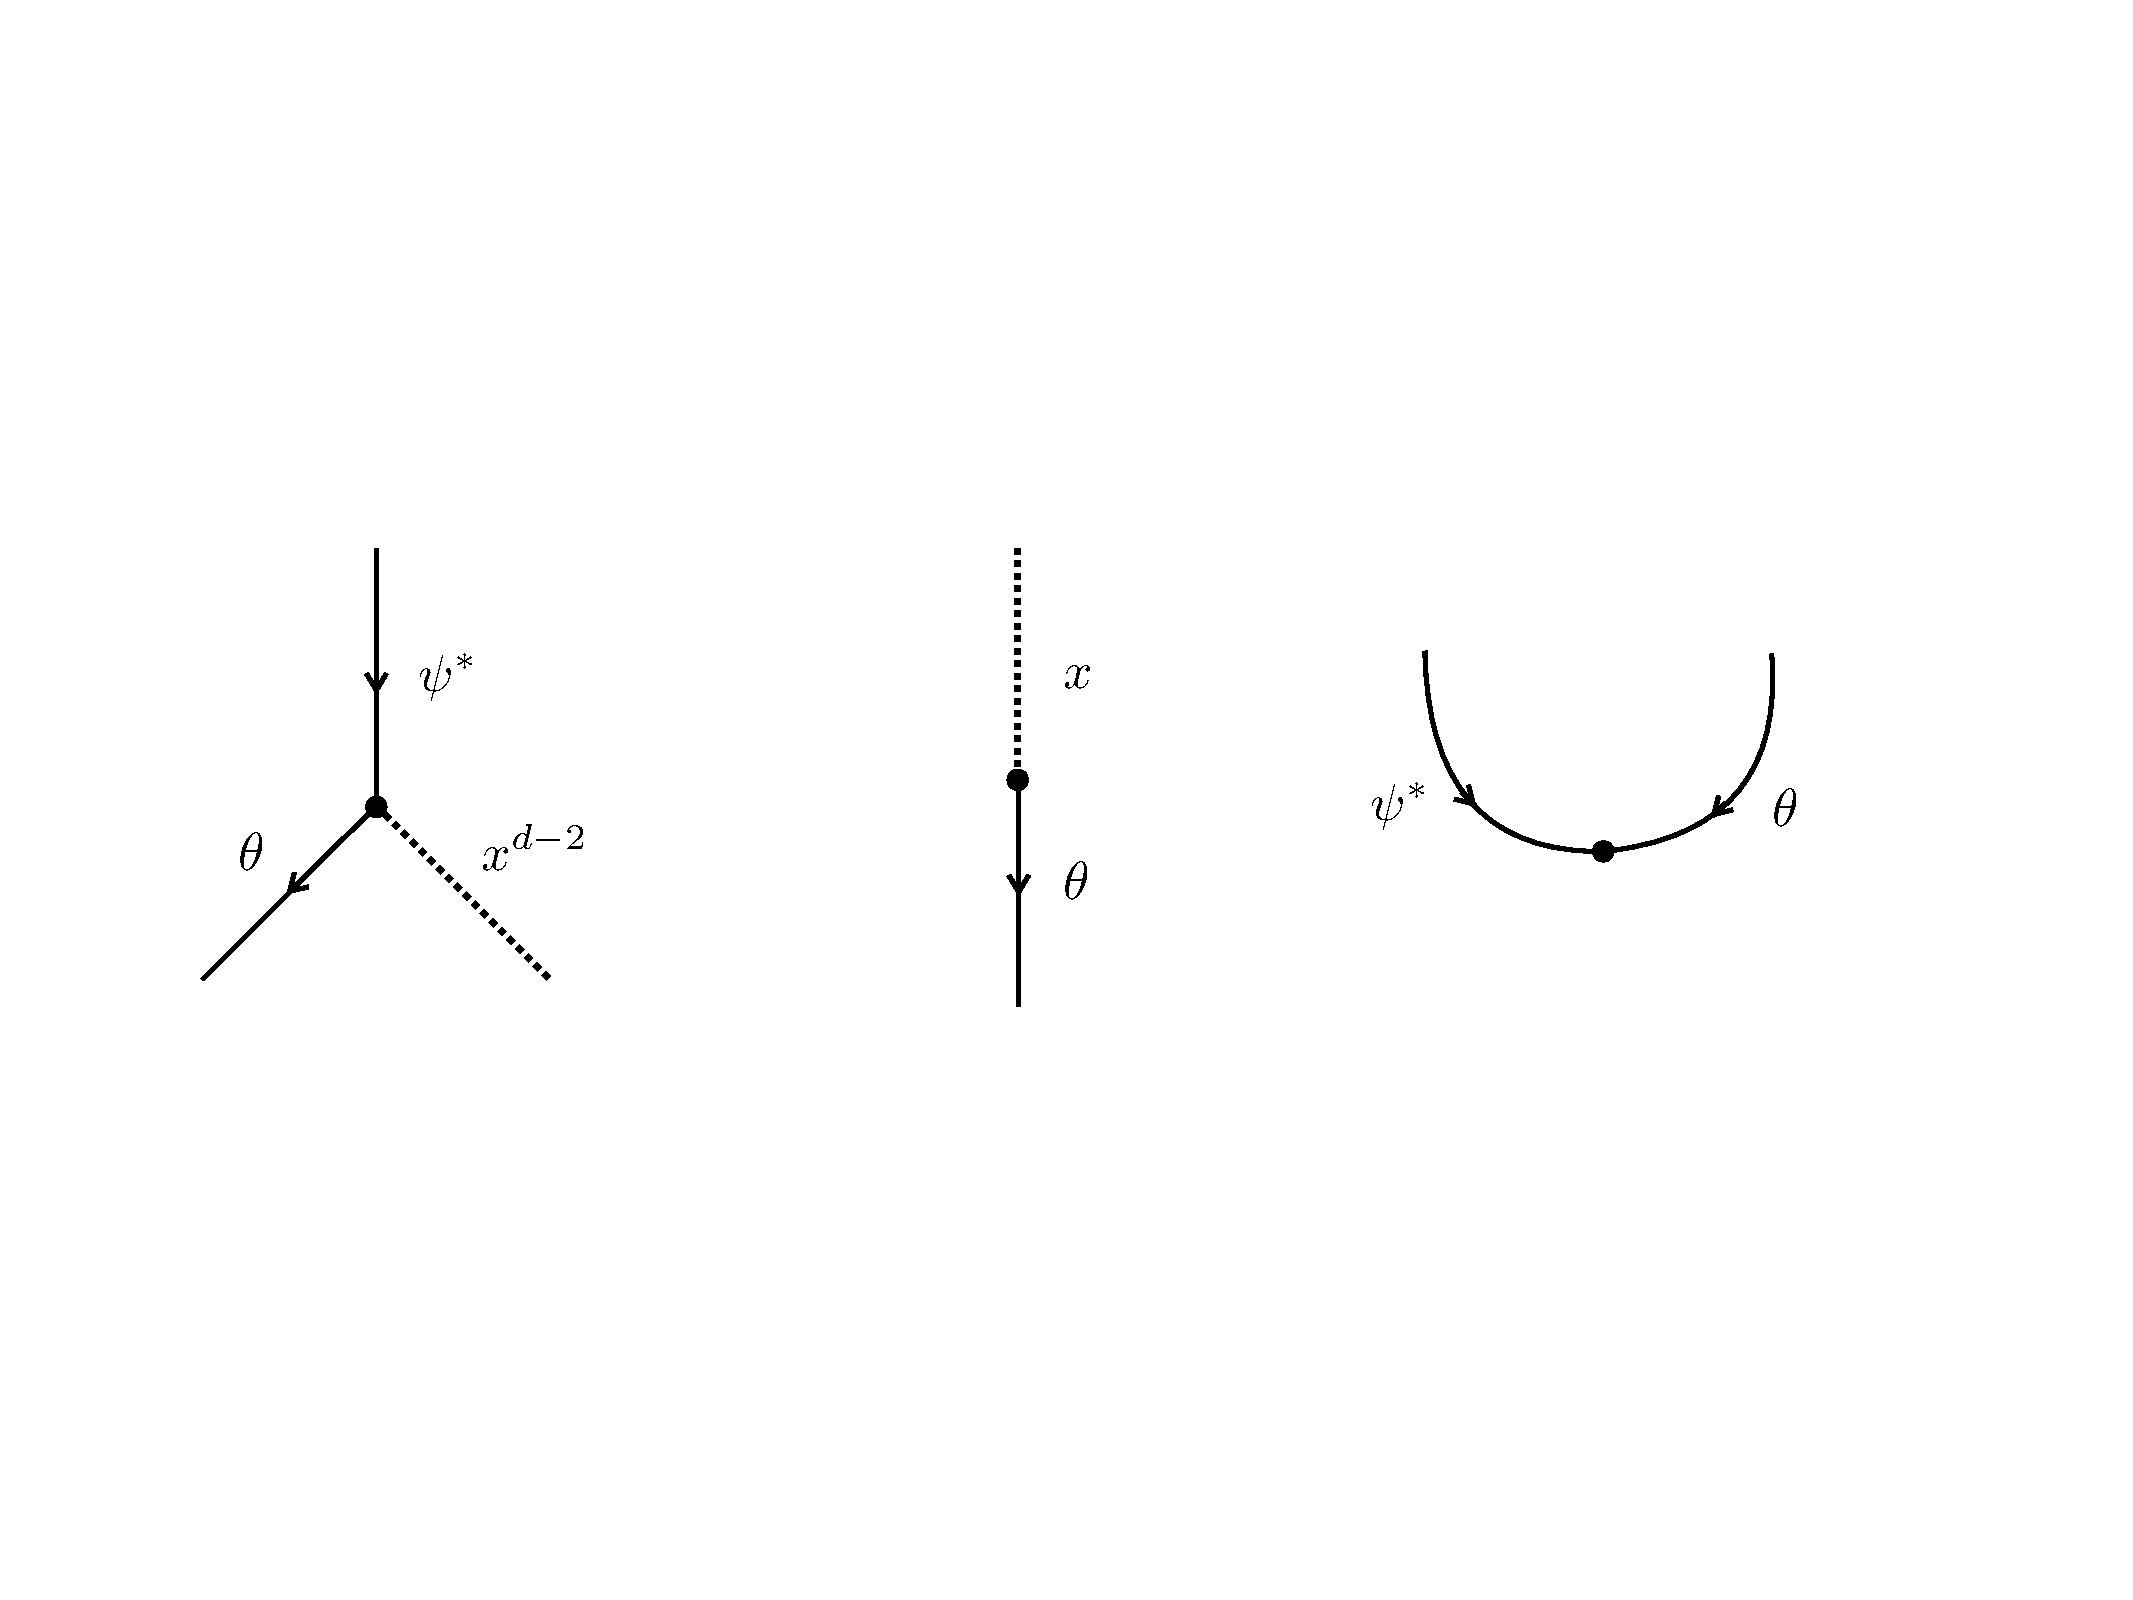
\includegraphics[scale=0.45]{dia9}
\end{center}
Let us compute the $A_\infty$-products $\rho_q$ on $\mathscr{B}$:
\begin{itemize}
\item For $q = 2$ there is only one tree $T \in \cat{T}_2$, which has no internal edge, and therefore no configuration $C$ containing an A-interaction (that is, $m(v) > 0$ at an input vertex) which contributes to $\rho_2$. So it is clear that
\be\label{eq:a_type_product}
\rho_2( \Lambda_2, \Lambda_1 ) = (-1)^{\widetilde{\Lambda_1} \widetilde{\Lambda_2} + \widetilde{\Lambda_1} + 1} \Lambda_1 \cdot \Lambda_2
\ee
where $(-) \cdot (-)$ denotes the usual product in the exterior algebra. This is just the forward suspension of the product in the exterior algebra.

\item For $q > 2$ let $C$ be a configuration with $\cat{O}(T,C) \neq 0$. Then $C$ must have at least one A-type interaction, since otherwise the $\partial_x$ in the B-type interactions are applied to $1 \in R$. Moreover, these A-type interactions can only be inserted at input vertices, since at an internal edge \eqref{eq:int_intedge} would contribute $\theta^2 = 0$.

For the same reason, the $\theta$ coming out of the B-type interaction at an internal edge $e$ must be consumed in a C-type interaction at the vertex $v$ immediately after $e$ on the path to the root: if not, it will annihilate with the $\theta$ emitted at the next internal edge, or, if $v$ is adjacent to the root, it will annihilate with $p$. This means that every edge $e$ must be the right-hand branch at $v$, from which we deduce that $T$ is the tree in which all internal edges lie on the path from the rightmost input to the root:
\begin{center}
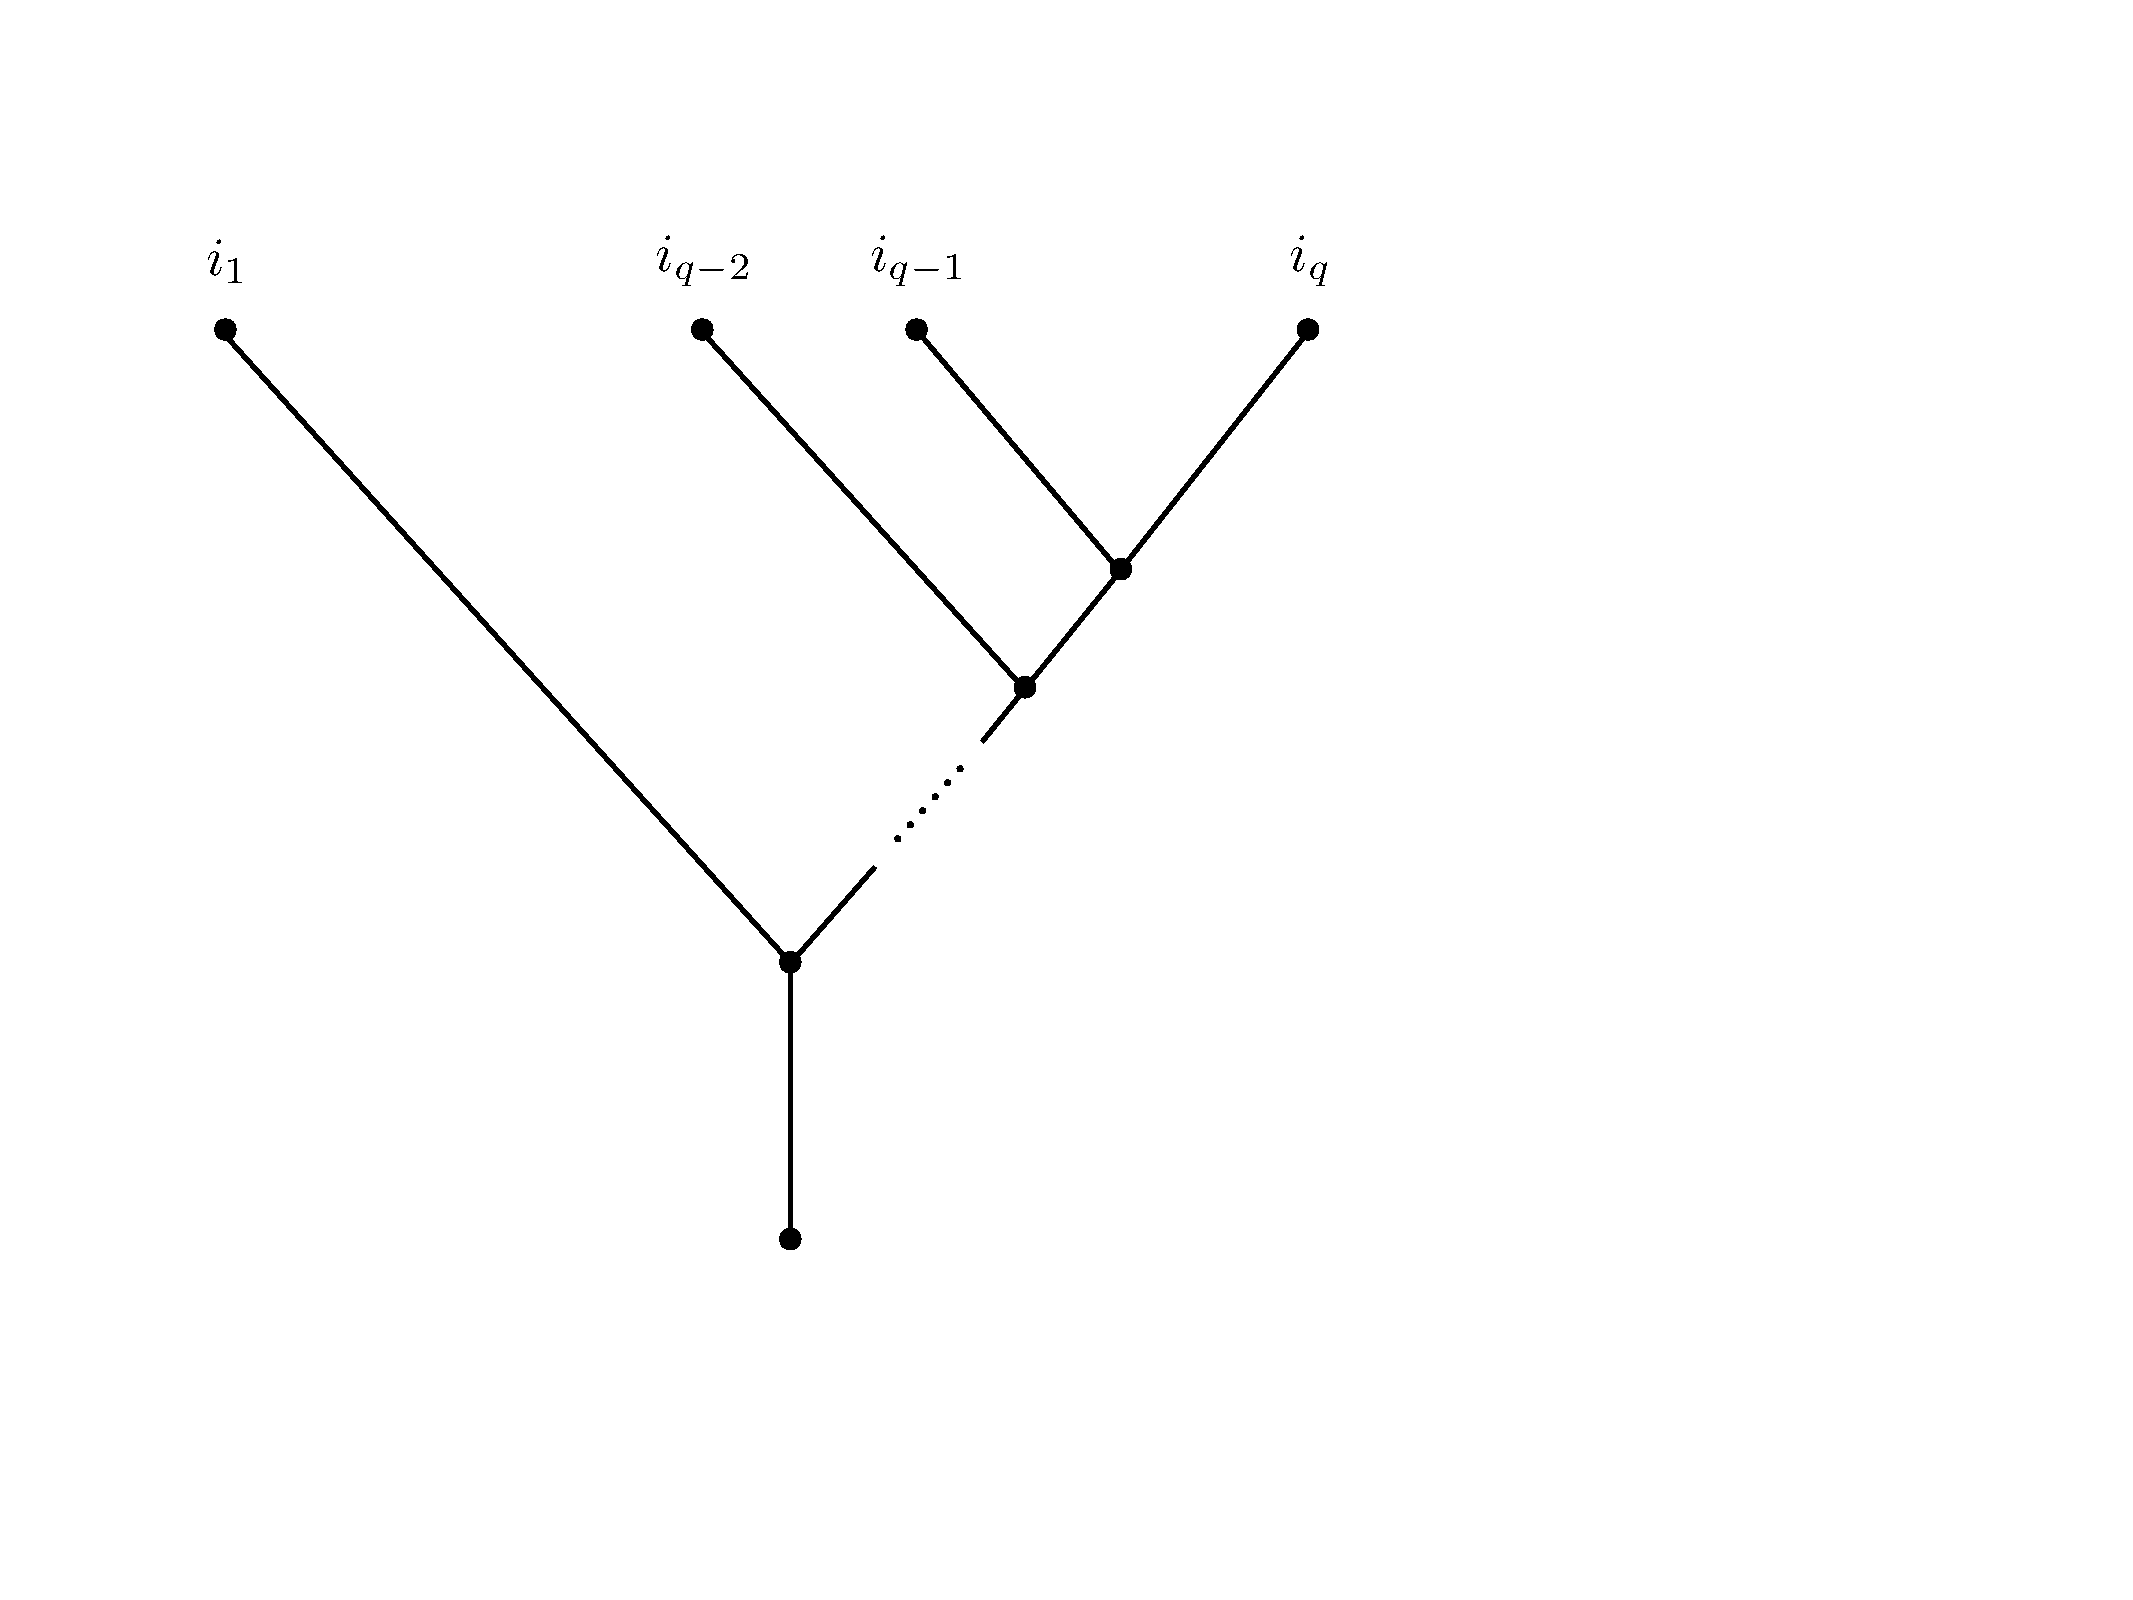
\includegraphics[scale=0.3]{dia10}
\end{center}
This implies that there is \emph{precisely} one A-type interaction in $C$, and it takes place at the vertex marked $i_q$ in the diagram. But since $T$ contains $q - 2$ internal edges, if $\cat{O}(T,C) \neq 0$ then we must have $q = d$. That is, $\rho_q = 0$ unless $q \in \{2,d\}$.

\item Finally, let us describe $\rho_d: \mathscr{B}^{\otimes d} \lto \mathscr{B}$ on the basis of tensors $(\psi^*)^{s_0} \otimes \cdots \otimes (\psi^*)^{s_d}$ where $s_j \in \{0,1\}$ for $1 \le j \le d$. We require a copy of $\psi^*$ at each input $i_1,\ldots,i_{q-2}$ in order to meet the $\theta$ emitted by B-type interactions, a copy of $\psi^*$ at $i_{q-1}$ to meet the $\theta$ from the A-type interaction and a $\psi^*$ at $i_q$ to initiate that A-type interaction. Hence $\rho_d$ is zero on all the basis elements except for
\[
\rho_d( \psi^* \otimes \psi^* \otimes \cdots \otimes \psi^* ) = (-1)^{Q(T, \underline{\Lambda})} \cdot 1\,.
\]
To compute the sign, observe that $e_i(T) = d - 2$ and $\Lambda_i = \psi^*$ is odd so $\widetilde{\Lambda_i}$ is even, whence $Q(T, \underline{\Lambda}) = (d-2) + d + 1 = 1$.
\end{itemize}
In summary: the underlying $\nZ_2$-graded $k$-module of $\mathscr{B}$ is the exterior algebra $\bigwedge( k \psi^* )$ and the $A_\infty$-products $\rho_q$ are zero unless $q \in \{ 2, d \}$. The product $\rho_2$ is the forward suspended version of the usual product on the exterior algebra, while
\[
\rho_d( \psi^* \otimes \psi^* \otimes \cdots \otimes \psi^* ) = -1\,.
\]
\end{example}

\section{Perturbation and Koszul complexes}

Let $k$ be a characteristic zero field, $R =  k[x_1,\ldots,x_n]$ and let $W \in \mf{m}^3$ be a potential with chosen decomposition $W = \sum_{i=1}^n x_i W^i$. We aim to construct the minimal model of the DG-algebra
\begin{align*}
\mathscr{A} &= \Big( \End_{R}(k^{\operatorname{stab}}), \; \partial = [d_{k^{\stab}},-] \; \Big)\\
&= \Big( R \otimes_k \End_k\Big( \bigwedge\big( \oplus_{i=1}^n k\psi_i \,\big) \Big),  \partial = \sum_i x_i [\psi_i^*,-] + \sum_i W^i [\psi_i,-] \;\Big)
\end{align*}
we first enlarge this DG-algebra to $S \otimes_k \mathscr{A}$, where $S$ is the exterior algebra
\be
S = \bigwedge\big( \oplus_{i=1}^n k\theta_i \,\big)
\ee
viewed as a $\nZ_2$-graded DG-algebra with grading $|\theta_i| = 1$ and zero differential. We also need to introduce the $nZ_2$-graded vector space
\be
\mathscr{E} = \End_k\Big( \bigwedge\big( \oplus_{i=1}^n k \psi_i \,\big) \Big)
\ee
and the Koszul complex of $x_1,\ldots,x_n$,
\be\label{eq:defnkoszulK}
K = \Big( R \otimes \bigwedge\big( \oplus_{i=1}^n k \theta_i \,\big), \; d_K = \sum_i x_i \theta_i^*\; \Big)
\ee
Note that $S \otimes_k \mathscr{A}$ has the same underlying $\nZ_2$-graded $k$-module as $K \otimes_R \mathscr{A}$.

\begin{theorem} There is a diagram of $k$-linear homotopy equivalences
\be\label{eq:first_he}
\xymatrix@C+3pc{
\big( S \otimes_k \mathscr{A}, \partial \,\big) \ar@<1ex>[r]^-{\exp(-\delta)} & \big( K \otimes_R \mathscr{A}, d_K + \partial \,\big) \ar@<1ex>[l]^-{ \exp(-\delta) } \ar@<1ex>[r]^-{\pi} & \big( \mathscr{E}, 0 \,\big)\,.\ar@<1ex>[l]^-{ \sigma_\infty }
}
\ee
\end{theorem}
\begin{proof}
See \cite{murfet}.
\end{proof}

The notation is as follows:
\begin{itemize}
\item The complexes involved here are
\begin{gather*}
\big( S \otimes \End_R(k^{\stab}), \; \partial \,\big)\\
\big( K \otimes_R \End_R(k^{\stab}), \; d_K + \partial\, \big)\\
\big( \md{E}, 0 \big)\,.
\end{gather*}
\item The operator $\psi_j = \psi_j \wedge -$ on $k^{\stab}$ satisfies
\[
[ \psi_j, d_{k^{\stab}} ] = \big[ \psi_j, \sum_i x_i \psi_i^* \big] = x_j \cdot 1\,,
\]
where $[-,-]$ always denotes the graded commutator. That is, $\psi_j$ is a homotopy for the action of $x_j$ on $k^{\stab}$. It is then easy to check that the odd operator $\alpha \mapsto \psi_j \circ \alpha$ on $\End_R(k^{\stab})$ is also a homotopy for $x_j$, and where it will not cause confusion we will also write $\psi_j$ for this operator of post-composition.

\item Both $S \otimes \md{A}_W$ and $K \otimes_R \md{A}_W$ have the same underlying $\nZ_2$-graded $k$-module, namely
\be\label{eq:same_underlying}
R \otimes \bigwedge( \oplus_{i=1}^n k\theta_i ) \otimes \End_k\big( \bigwedge( \oplus_{i=1}^n k \psi_i ) \big)\,.
\ee
On this space we define the even operator
\be
\delta = \sum_{i=1}^n \psi_i \theta_i^*\,,
\ee
where $\psi_i$ is the operator on $\End_R(k^{\stab})$ discussed above, given by $\alpha \mapsto (\psi_i \wedge -) \circ \alpha$, and $\theta_i^*$ acts by contraction on $S$. It is easy to check that $\exp(\delta),\exp(-\delta)$ intertwines the differentials $\partial$ and $d_K + \partial$ and therefore gives an isomorphism between the first two complexes in \eqref{eq:first_he} \cite[Proposition 4.11]{murfet}.
\item The morphism of complexes $\pi: K \lto R/\mf{m}$ is defined by composing the projection of $K$ onto the submodule $R \cdot 1$ of $\theta$-degree zero forms, with the quotient $R \lto R/\mf{m}$. We also write $\pi$ for the result of tensoring this morphism with $\End_R(k^{\stab})$ to obtain
\[
\xymatrix@C+2pc{
K \otimes_R \End_R(k^{\stab}) \ar[r]^-{\pi \otimes 1} & R/\mf{m} \otimes_R \End_R(k^{\stab}) = \underline{\End}(k^{\stab})\,.
}
\]
This is a morphism of complexes, because the differential on $\End_R(k^{\stab})$ vanishes on the quotient $\underline{\End}(k^{\stab})$ by the hypothesis that $W \in \mf{m}^2$.
\item The $k$-linear homotopy inverse $\sigma_\infty$ to $\pi$ in \eqref{eq:first_he} is defined in terms of the following ingredients. The first is the $k$-linear connection (viewing $\theta_i$ as a $1$-form)
\be
\nabla: K \lto K\,, \qquad \nabla = \sum_i \partial_{i} \theta_i
\ee
and the degree $-1$ (with respect to the $\theta$-degree) $k$-linear operator
\be
H = [d_K, \nabla]^{-1} \nabla\,.
\ee
We write $\partial$ for the differential on $\End_R(k^{\stab})$, and $\sigma: k \lto K$ for the map which sends $\lambda \in k$ to $\lambda \cdot 1 \in K$, and define $k$-linear maps
\begin{align}
\sigma_\infty = \sum_{m \ge 0} (-1)^m (H \partial)^m \sigma\,,\\
H_\infty = \sum_{m \ge 0} (-1)^m (H \partial)^m H\,.
\end{align}
Here $H_\infty$ is an odd operator on $K \otimes_R \End_R(k^{\stab})$. These maps satisfy:
\begin{align}
\pi \sigma_\infty &= 1\,,\\
 \sigma_\infty \pi &= 1 - [d_K + \partial, H_\infty]\,.
\end{align}
\end{itemize}

By inspection of \eqref{eq:first_he}, we therefore have the following:

\begin{proposition}\label{prop:he_start} There is a diagram of morphisms of $\nZ_2$-graded $k$-complexes
\be\label{eq:he_start}
\xymatrix@C+5pc{
S \otimes \md{A}_W \ar@<1ex>[r]^-{\Phi} & \md{E}\ar@<1ex>[l]^-{\Phi^{-1}}
}
\ee
where $\Phi = \pi \exp(-\delta), \Phi^{-1} = \exp(\delta) \sigma_\infty$ and $\widehat{H} = \exp(\delta) H_\infty \exp(-\delta)$ satisfy
\be
\Phi \Phi^{-1} = 1\,, \qquad \Phi^{-1} \Phi = 1 - [\partial, \widehat{H}]\,.
\ee
Thus, $\Phi$ and $\Phi^{-1}$ are mutually inverse homotopy equivalences over $k$.
\end{proposition}

The endomorphism algebra $C = \End_k(S)$ is a Clifford algebra generated by the contraction $\theta_i^*$ and wedge product $\theta_i$ operators. It is observed in \cite{murfet} that \eqref{eq:he_start} is an isomorphism of Clifford representations (in the homotopy category) when the complex $\md{E}$ is equipped with the action induced by Atiyah classes:

\begin{definition}
The Atiyah classes of $\md{A}_W$ are the $R$-linear odd operators
\[
\At_i = [\partial, \partial_{i}]: \End_R(k^{\stab}) \lto \End_R(k^{\stab})\,,
\]
\end{definition}

\begin{lemma} We have
\[
\At_i = -[\psi_i^*, -] - \sum_{q=1}^n \partial_{i}(W^q) [ \psi_q, - ]\,.
\]
\end{lemma}
\begin{proof}
By direct calculation:
\begin{align*}
\At_i &= \big[ [d_{k^{\stab}},-], \partial_{i} \big]\\
&= \sum_q \big[x_q [\psi_q^*,-], \partial_{i}\big] + \sum_q \big[W^q [\psi_q,-], \partial_{i}\big]\\
&= -\sum_q \partial_{i}(x_q) [\psi_q^*,-] - \sum_q \partial_{i}(W^q) [\psi_q,-]\\
&= -[\psi_i^*,-] - \sum_q \partial_{i}(W^q) [\psi_q, -]\,.
\end{align*}
\end{proof}

\begin{lemma} The induced Clifford algebra structure on $\mathscr{E}$ is given by
\[
\gamma_i^\dagger = \At_i = -[\psi_i^*, -]\,, \qquad \gamma_i = -\psi_i\,.
\]
\end{lemma}

\begin{lemma} The idempotent $e = \gamma_1^\dagger \cdots \gamma_n^\dagger \gamma_n \cdots \gamma_1$ is the projection onto $\mathscr{B} \subseteq \mathscr{E}$.
\end{lemma}

We define the even operator $\delta_i = \psi_i \theta_i^*$ on the underlying module $\eqref{eq:same_underlying}$ of $S \otimes \md{A}_W$, so that $\delta = \sum_i \delta_i$. Since $[ \delta_i, \delta_j ] = 0$ for all $i,j$ we have
\be
\exp(\pm \delta) = \exp(\pm \delta_1) \cdots \exp(\pm \delta_n)\,.
\ee

\begin{lemma} For $1 \le i \le n$ there is a commutative diagram
\be
\xymatrix@C+3pc@R+1pc{
(S \otimes \md{A}_W) \otimes (S \otimes \md{A}_W) \ar[d]_-{\delta_i \otimes 1 + 1 \otimes \delta_i + [\psi_i,-] \otimes \theta_i^*} \ar[r]^-{m_2} & S \otimes \md{A}_W \ar[d]^-{\delta_i}\\
(S \otimes \md{A}_W) \otimes (S \otimes \md{A}_W) \ar[r]_-{m_2} & S \otimes \md{A}_W
}
\ee
\end{lemma}

\begin{definition} We define
\be
\Xi_i = [ \psi_i, - ] \otimes \theta_i^* : S \otimes \md{A}_W \lto S \otimes \md{A}_W\,.
\ee
and
\be
\Xi = \sum_i \Xi_i\,.
\ee
\end{definition}

\begin{proposition} There is a commutative diagram
\be
\xymatrix@C+3pc@R+2pc{
(S \otimes \md{A}_W) \otimes (S \otimes \md{A}_W) \ar[d]_-{\exp(-\delta) \otimes \exp(-\delta)} \ar[r]^-{m_2} & S \otimes \md{A}_W \ar[dd]^-{\exp(-\delta)}\\
(S \otimes \md{A}_W) \otimes (S \otimes \md{A}_W) \ar[d]_-{\exp(-\Xi)}\\
(S \otimes \md{A}_W) \otimes (S \otimes \md{A}_W) \ar[r]_-{m_2} & S \otimes \md{A}_W
}
\ee
\end{proposition}

\newpage

We have for $m > 0$, as an operator on $\mathscr{H}$
\begin{align*}
\big( H \partial )^m &= \prod_{i=1}^m \sum_{j_i = 1}^n H \Big( x_{j_i} [\psi_{j_i}^*,-] + W^{j_i} [\psi_{j_i},-] \Big)\,.
\end{align*}
Prior to Definition \ref{defn:otc} we observed that in calculating $\langle D_{T,C} \rangle$ it suffices to consider operators on the smaller $\nZ_2$-graded $k$-module
\be
\mathscr{H}' = R \otimes_k \bigwedge\big( \oplus_{i=1}^n k \theta_i \,\big) \otimes_k \mathscr{B}\,.
\ee
On this submodule of $\mathscr{H}$ the operators $[\psi_i^*,-]$ act as zero, and so $(H \partial)^m$ takes a simpler form. If $\underline{j}$ ranges over elements in of $\{1,\ldots,n\}^m$ and $\underline{\gamma}$ over elements of $(\mathbb{N}^n)^m$ then
\begin{align*}
\big( H \partial )^m \arrowvert_{\mathscr{H}'} &= \sum_{\underline{j}} \prod_{i=1}^m H \Big( W^{j_i} [ \psi_{j_i}, - ] \Big)\\
&= \sum_{\underline{j}, \underline{\gamma}} \prod_{i=1}^m H \Big( W^{j_i}(\gamma_i) x^{\gamma_i} [ \psi_{j_i}, - ] \Big)\\
&= \sum_{\underline{j}, \underline{\gamma}} \prod_{i=1}^m [d_K, \nabla]^{-1} \nabla \Big( W^{j_i}(\gamma_i) x^{\gamma_i} [ \psi_{j_i}, - ] \Big)\,.
\end{align*}
Note that $W^i$ contains no constant term, since by hypothesis $W \in \mf{m}^2$. Our convention is that products of operators expand from left to right as $i$ increases, so that the rightmost factor in the product is $i = m$. Recall that $\nabla = \sum_i \partial_i \theta_i$ and $[d_K, \nabla]$ acts on a tensor product $f \otimes \omega$, where $f$ and $\omega$ are homogeneous, by
\[
[d_K, \nabla]( f \otimes \omega ) = ( |f| + |\omega| ) f \otimes \omega\,.
\]
Now we consider the scalar factors produced by the $[d_K, \nabla]^{-1}$ when we apply $(H \partial)^m$ to a tensor $f \otimes \omega \otimes \Psi$. Observe how the sum of the polynomial and $\theta$-degree changes with each application of $H \partial$. Multiplying with $x^{\gamma_i}$ increases the polynomial degree by $|\gamma_i|$, while applying $\nabla$ decreases the polynomial degree and increases the $\theta$-degree by one, so overall the $i$th copy of $H \partial$ (reading from left to right) increases the sum of the two degrees from
\[
|f| + |\omega| + \sum_{t > i} |\gamma_t| \qquad \text{ to } \qquad |f| + |\omega| + \sum_{t \ge i} |\gamma_t|\,.
\]
If we write $a = |f| + |\omega|$ then the scalar factor contributed by the copies of $[d_K, \nabla]^{-1}$ in $(H \partial)^m$ applied to $f \otimes \omega \otimes \Psi$ is therefore
\[
\frac{1}{(a + |\gamma_m|)(a + |\gamma_m| + |\gamma_{m-1}|) \cdots (a + |\gamma_m| + \cdots + |\gamma_1|)}\,.
\]
This leads us to the un-symmetrised version of $\zeta$ from Definition \ref{defn:zeta}:

\begin{definition} Given a sequence $a_1,\ldots,a_m \ge 1$ of integers and $a \ge 0$ we define
\be
\zeta_a(a_1,\ldots,a_m) = \frac{1}{(a + a_m)(a + a_{m-1} + a_m) \cdots (a + a_1 + \cdots + a_m)}\,.
\ee
\end{definition}

Let $\mathscr{H}'_a \subseteq \mathscr{H}$ denote the submodule of elements of degree $a$, when we take the $\nZ$-grading induced by the usual $\nZ$-grading on $R$ and the exterior algebra in the $\theta$'s (so, the grading does not count $\psi$'s). Then we have computed that
\be
(H \partial)^m|_{\mathscr{H}'_a} = \sum_{\underline{j}, \underline{\gamma}} \zeta_{a}( |\gamma_1|, \ldots, |\gamma_m| ) \Big\{ \prod_{i=1}^m \nabla \circ \big( W^{j_i}(\gamma_i)x^{\gamma_i} [ \psi_{j_i}, - ] \big) \Big\} \,.
\ee
Now let $\Ker(\nabla)$ denote the kernel of $\nabla$ acting on $\mathscr{H}$. Since $\nabla^2 = 0$ and
\be
[ \nabla, f[ \psi, - ] ] = - \sum_q \partial_q(f) [\psi,-] \theta_q
\ee
we have
\begin{align*}
\big( H \partial )^m|_{\mathscr{H}'_a \cap \Ker(\nabla)} &= \sum_{\underline{j}, \underline{\gamma}} \zeta_{a}( |\gamma_1|, \ldots, |\gamma_m| ) \Big\{ \prod_{i=1}^m \Big[ \nabla, W^{j_i}(\gamma_i)x^{\gamma_i} [ \psi_{j_i}, - ] \Big]\Big\}\\
&= \sum_{\underline{j}, \underline{\gamma},\underline{z}} (-1)^m \zeta_{a}( |\gamma_1|, \ldots, |\gamma_m| ) \Big\{\prod_{i=1}^m W^{j_i}(\gamma_i) \partial_{z_i}(x^{\gamma_i}) [ \psi_{j_i}, - ] \theta_{z_i} \Big\}
\end{align*}
where $\underline{z}$ ranges over $\{1, \ldots, n\}^m$.

\begin{remark}\label{remark:virt_part_2} Continuing from Remark \ref{remark:virtual_part} we note that in constrast to the the way we usually think about the minimal model construction in the setting of topological string theory \cite{??} the elements $\Psi$ of $\mathscr{B}$ are not immediately identified with cohomology classes of $\mathscr{B}$. 

Of course $\sigma_\infty(\Psi)$ is a cycle for $\partial$, but this is already given by a complicated sum which contributes multiple Feynman diagrams in the calculus of Definition \ref{??}. That is to say, we have found it useful for purposes of calculation to have the incoming states in our Feynman diagrams to be elements of $\mathscr{H}$ that are \emph{not} cycles. Note that as we vary the potential $W$ the elements of $\mathscr{H}$ that are cycles will change - this makes it awkward to take as a starting point the cohomology of $\mathscr{H}$. In our approach the subspace $\mathscr{B}$ remains fixed, and even in the case of quadratic terms it is only the projection to $\mathscr{B}$ that changes.
\end{remark}

\begin{remark} See ainfmf12 for idempotents.
\end{remark}

\newpage

\bibliographystyle{amsalpha}
\providecommand{\bysame}{\leavevmode\hbox to3em{\hrulefill}\thinspace}
\providecommand{\href}[2]{#2}
\begin{thebibliography}{BHLS03}
  
  \bibitem[Dyc11]{d0904.4713}
T.~Dyckerhoff, \textsl{Compact generators in categories of matrix factorizations},
  Duke Math. J. \textbf{159} (2011), 223--274,
  \href{http://arxiv.org/abs/0904.4713}{[arXiv:0904.4713]}.
  
\bibitem{lazaroiu}
C.~I.~Lazaroiu, \textsl{Generating the superpotential on a D-brane category: I}, [arXiv:hep-th/0610120].

\bibitem{lazaroiu2}
C.~I.~Lazaroiu, \textsl{String field theory and brane superpotentials}.
  
\bibitem{murfet}
D.~Murfet, \textsl{Computing with cut systems}, \href{http://arxiv.org/abs/1402.4541}{[arXiv:1402.4541]}.

\bibitem{lgdual}
N.~Carqueville and D.~Murfet, \textsl{Adjunctions and defects in Landau-Ginzburg models}, Adv. Math. \textbf{289} (2016), 480--566.

\bibitem{dm1102.2957}
T.~Dyckerhoff and D.~Murfet, \textsl{Pushing forward matrix factorisations}, Duke Math. J. \textbf{162} (2013), 1249--1311.

\bibitem{weinberg}
Weinberg, \textsl{The Quantum Theory of Fields Volume 1}.

\bibitem{ps}
Peskin \& Shroeder, \textsl{An introduction to QFT}.

\bibitem{sullivan}
D.~Sullivan, \textsl{Open and closed string field theory interpreted in classical algebraic topology} London Math. Soc. Lecture Note Series 308 (2004).

\end{thebibliography}

\end{document}